\documentclass[twoside]{book}

% Packages required by doxygen
\usepackage{fixltx2e}
\usepackage{calc}
\usepackage{doxygen}
\usepackage[export]{adjustbox} % also loads graphicx
\usepackage{graphicx}
\usepackage[utf8]{inputenc}
\usepackage{makeidx}
\usepackage{multicol}
\usepackage{multirow}
\PassOptionsToPackage{warn}{textcomp}
\usepackage{textcomp}
\usepackage[nointegrals]{wasysym}
\usepackage[table]{xcolor}

% Font selection
\usepackage[T1]{fontenc}
\usepackage[scaled=.90]{helvet}
\usepackage{courier}
\usepackage{amssymb}
\usepackage{sectsty}
\renewcommand{\familydefault}{\sfdefault}
\allsectionsfont{%
  \fontseries{bc}\selectfont%
  \color{darkgray}%
}
\renewcommand{\DoxyLabelFont}{%
  \fontseries{bc}\selectfont%
  \color{darkgray}%
}
\newcommand{\+}{\discretionary{\mbox{\scriptsize$\hookleftarrow$}}{}{}}

% Page & text layout
\usepackage{geometry}
\geometry{%
  a4paper,%
  top=2.5cm,%
  bottom=2.5cm,%
  left=2.5cm,%
  right=2.5cm%
}
\tolerance=750
\hfuzz=15pt
\hbadness=750
\setlength{\emergencystretch}{15pt}
\setlength{\parindent}{0cm}
\setlength{\parskip}{3ex plus 2ex minus 2ex}
\makeatletter
\renewcommand{\paragraph}{%
  \@startsection{paragraph}{4}{0ex}{-1.0ex}{1.0ex}{%
    \normalfont\normalsize\bfseries\SS@parafont%
  }%
}
\renewcommand{\subparagraph}{%
  \@startsection{subparagraph}{5}{0ex}{-1.0ex}{1.0ex}{%
    \normalfont\normalsize\bfseries\SS@subparafont%
  }%
}
\makeatother

% Headers & footers
\usepackage{fancyhdr}
\pagestyle{fancyplain}
\fancyhead[LE]{\fancyplain{}{\bfseries\thepage}}
\fancyhead[CE]{\fancyplain{}{}}
\fancyhead[RE]{\fancyplain{}{\bfseries\leftmark}}
\fancyhead[LO]{\fancyplain{}{\bfseries\rightmark}}
\fancyhead[CO]{\fancyplain{}{}}
\fancyhead[RO]{\fancyplain{}{\bfseries\thepage}}
\fancyfoot[LE]{\fancyplain{}{}}
\fancyfoot[CE]{\fancyplain{}{}}
\fancyfoot[RE]{\fancyplain{}{\bfseries\scriptsize Generated by Doxygen }}
\fancyfoot[LO]{\fancyplain{}{\bfseries\scriptsize Generated by Doxygen }}
\fancyfoot[CO]{\fancyplain{}{}}
\fancyfoot[RO]{\fancyplain{}{}}
\renewcommand{\footrulewidth}{0.4pt}
\renewcommand{\chaptermark}[1]{%
  \markboth{#1}{}%
}
\renewcommand{\sectionmark}[1]{%
  \markright{\thesection\ #1}%
}

% Indices & bibliography
\usepackage{natbib}
\usepackage[titles]{tocloft}
\setcounter{tocdepth}{3}
\setcounter{secnumdepth}{5}
\makeindex

% Hyperlinks (required, but should be loaded last)
\usepackage{ifpdf}
\ifpdf
  \usepackage[pdftex,pagebackref=true]{hyperref}
\else
  \usepackage[ps2pdf,pagebackref=true]{hyperref}
\fi
\hypersetup{%
  colorlinks=true,%
  linkcolor=blue,%
  citecolor=blue,%
  unicode%
}

% Custom commands
\newcommand{\clearemptydoublepage}{%
  \newpage{\pagestyle{empty}\cleardoublepage}%
}

\usepackage{caption}
\captionsetup{labelsep=space,justification=centering,font={bf},singlelinecheck=off,skip=4pt,position=top}

%===== C O N T E N T S =====

\begin{document}

% Titlepage & ToC
\hypersetup{pageanchor=false,
             bookmarksnumbered=true,
             pdfencoding=unicode
            }
\pagenumbering{roman}
\begin{titlepage}
\vspace*{7cm}
\begin{center}%
{\Large sym-\/ildl \\[1ex]\large 1.\+2 }\\
\vspace*{1cm}
{\large Generated by Doxygen 1.8.11}\\
\end{center}
\end{titlepage}
\clearemptydoublepage
\tableofcontents
\clearemptydoublepage
\pagenumbering{arabic}
\hypersetup{pageanchor=true}

%--- Begin generated contents ---
\chapter{\textbackslash{}authors $<$a href=\char`\"{}https\+://www.\+cs.\+ubc.\+ca/$\sim$greif/\char`\"{}$>$Chen Greif$<$/a$>$, Shiwen He, $<$a href=\char`\"{}https\+://www.\+cs.\+ubc.\+ca/$\sim$inutard/\char`\"{}$>$Paul Liu$<$/a$>$}
\label{index}\hypertarget{index}{}\hypertarget{index_intro_sec}{}\section{Overview}\label{index_intro_sec}
{\bfseries sym-\/ildl} is a C++ package for solving and producing fast incomplete factorizations of symmetric indefinite or skew-\/symmetric matrices. Given an $n\times n$ symmetric indefinite or skew-\/symmetric matrix $\mathbf{A}$, this package produces an incomplete $\mathbf{LDL^{T}}$ factorization. Prior to factorization, {\bfseries sym-\/ildl} first scales the matrix to be equilibrated in the max-\/norm \href{#refs}{\tt \mbox{[}2\mbox{]}}, and then preorders the matrix using either the Reverse Cuthill-\/\+Mc\+Kee (R\+CM) algorithm or the Approximate Minimum Degree algorithm (A\+MD) \href{#refs}{\tt \mbox{[}1\mbox{]}}. To maintain stability, the user can use Bunch-\/\+Kaufman or rook partial pivoting during the factorization process. The factorization produced is of the form \[ \mathbf{P^{T}SASP \approx LDL^{T}}. \] where $\mathbf{P}$ is a permutation matrix, $\mathbf{S}$ a scaling matrix, and $\mathbf{L}$ and $\mathbf{D}$ are the unit lower triangular and block diagonal factors respectively. The user can also optionally solve the given linear system, using {\bfseries sym-\/ildl\textquotesingle{}s} incomplete factorization to precondition the built-\/in solver or using the full factorization as a direct solver.

This package is based on and extends an incomplete factorization approach proposed by Li and Saad \href{#refs}{\tt \mbox{[}3\mbox{]}} (which itself builds on Li, Saad, and Chow \href{#refs}{\tt \mbox{[}4\mbox{]}}).\hypertarget{index_dlinks}{}\section{Download links}\label{index_dlinks}
{\itshape \mbox{[}Latest release\+: 11/15/2015\mbox{]}} \hypertarget{index_matlab_dlinks}{}\subsection{M\+A\+T\+L\+A\+B M\+E\+X Files}\label{index_matlab_dlinks}

\begin{DoxyItemize}
\item \href{https://github.com/inutard/matrix-factor/raw/master/release/win64/ildl-2015a.zip}{\tt For M\+A\+T\+L\+AB 2015a and above on 64-\/bit Windows 8.\+1}
\item \href{https://github.com/inutard/matrix-factor/raw/master/release/linux/ildl-2014a.zip}{\tt For M\+A\+T\+L\+AB 2014a and above on 64-\/bit Open\+S\+U\+SE 13.\+1} 
\end{DoxyItemize}\hypertarget{index_binary_dlinks}{}\subsection{Prebuilt binaries}\label{index_binary_dlinks}

\begin{DoxyItemize}
\item \href{https://github.com/inutard/matrix-factor/raw/master/release/win64/ldl_driver.exe}{\tt For 64-\/bit Windows 8.\+1}
\item \href{https://github.com/inutard/matrix-factor/raw/master/release/linux/ldl_driver}{\tt For 64-\/bit Open\+S\+U\+SE 13.\+2} 
\end{DoxyItemize}\hypertarget{index_source_dlinks}{}\subsection{The source code}\label{index_source_dlinks}

\begin{DoxyItemize}
\item \href{https://github.com/inutard/matrix-factor/archive/master.zip}{\tt Latest stable release (gcc 4.\+7 and above)}
\end{DoxyItemize}\hypertarget{index_why_use}{}\section{Why use sym-\/ildl?}\label{index_why_use}

\begin{DoxyItemize}
\item {\bfseries It\textquotesingle{}s easy to use}\+: We offer precompiled versions of sym-\/ildl on both Windows and Linux, as well as for use within M\+A\+T\+L\+AB. If you want to use sym-\/ildl as a C++ library, there is no need to compile anything. You can just use the header files right away. sym-\/ildl is defined entirely in the header files.
\item {\bfseries It\textquotesingle{}s reliable}\+: sym-\/ildl includes several methods to improve stability of the preconditioner. These include different kinds of equilibration, reordering, as well partial pivoting.
\item {\bfseries It\textquotesingle{}s not just a preconditioner}\+: sym-\/ildl implements a direct solver as well as several iterative solvers that are integrated with the preconditioner, allowing you to easily and quickly solve your linear system.
\end{DoxyItemize}\hypertarget{index_quick_start}{}\section{Quick Start}\label{index_quick_start}
To begin using the package, first download the files above or compile the code hosted at \href{https://github.com/inutard/matrix-factor}{\tt https\+://github.\+com/inutard/matrix-\/factor}. The Git\+Hub repository contains the most up to date source code as well as an \char`\"{}experimental\char`\"{} branch that we release new features to. The package works under most Unix distributions as well as Cygwin under Windows. The default compiler used is {\ttfamily g++}, simply type {\ttfamily make} at the command line to compile the entire package. In addition to \hyperlink{index_ldl_driver}{usage as a standalone program}, the package also has a \hyperlink{index_matlab_mex}{Matlab interface}.

For using sym-\/ildl as a software library, see the A\+PI \href{http://www.cs.ubc.ca/~inutard/html/classsolver.html}{\tt here}. sym-\/ildl is a header only library, so one only needs to include {\ttfamily \hyperlink{solver_8h_source}{source/solver.\+h}} for everything to work.\hypertarget{index_ldl_driver}{}\subsection{Using the package as a standalone program}\label{index_ldl_driver}
The compiled program {\ttfamily ldl\+\_\+driver} takes in through the command line one parameter (the matrix) as well as several additional optional parameters.

The format of execution is\+: 
\begin{DoxyCode}
./ldl\_driver -filename=[matrix-name.mtx] [-rhs\_file=rhs-name.mtx ...]
\end{DoxyCode}


The parameters can be given in any order, and will use a default value when not specified.

A description of each of these parameters can be accessed by typing 
\begin{DoxyCode}
./ldl\_driver --help 
\end{DoxyCode}


Generally speaking, the code operates in two phases\+: generating the preconditioner (factorization) and solving the linear system (solver). The factorization parameters can be used to specify how the L\+DL\textquotesingle{} preconditioner is built. If a right hand side is specified, the built-\/in solver attempts to solve the given linear system. The solver takes the preconditioner and uses it in either preconditioned M\+I\+N\+R\+ES or a direct solve (full factorization with Bunch-\/\+Kaufman or rook pivoting).

For convenience, the parameters are listed below.\hypertarget{index_fact_param}{}\subsubsection{Factorization parameters}\label{index_fact_param}

\begin{DoxyParams}{Parameters}
{\em filename} & The filename of the matrix to be loaded. Several test matrices exist in the test\+\_\+matrices folder. All matrices loaded are required to be in matrix market (.mtx) form.\\
\hline
{\em fill} & Controls memory usage. Each column of $\mathbf{L}$ is guaranteed to have fewer than $fill\cdot nnz(\mathbf{A})/n$ elements. Each column of $\mathbf{D}$ has at most 2 elements. When this argument is not given, the default value for {\ttfamily fill} is {\ttfamily 3.\+0}.\\
\hline
{\em tol} & Controls agressiveness of dropping. In each column k, elements less than $tol \cdot \left|\left|\mathbf{L}_{k+1:n,k}\right|\right|_1$ are dropped. The default value for {\ttfamily tol} is {\ttfamily 0.\+001}.\\
\hline
{\em pp\+\_\+tol} & A parameter to aggressiveness of Bunch-\/\+Kaufman pivoting (B\+KP). When pp\+\_\+tol is 0, there is no partial pivoting. Values between 0 and 1 vary the number of pivots of B\+KP makes. When pp\+\_\+tol is equal to 1, standard B\+KP is used. The pp\+\_\+tol parameter is ignored if the pivot parameter is set to \textquotesingle{}rook\textquotesingle{}. See the {\bfseries pivot} parameters for more details. The default is \textquotesingle{}rook\textquotesingle{}.\\
\hline
{\em reordering} & Determines what sort of preordering will be used on the matrix. Choices are \textquotesingle{}amd\textquotesingle{}, \textquotesingle{}rcm\textquotesingle{}, and \textquotesingle{}none\textquotesingle{}. The default is \textquotesingle{}amd\textquotesingle{}.\\
\hline
{\em inplace} & Indicates whether the factorization should be performed in-\/place, leading to roughly a 33\% saving in memory. This memory comes out of extra information used in the solver. If the solver is needed, then {\ttfamily inplace} should not be used. {\ttfamily y} indicates yes, {\ttfamily n} indicates no. The default flag is {\ttfamily n}.\\
\hline
{\em pivot} & Indicates the pivoting algorithm used. Choices are \textquotesingle{}rook\textquotesingle{} and \textquotesingle{}bunch\textquotesingle{}. If {\ttfamily rook} is used, the {\ttfamily pp\+\_\+tol} parameter is ignored. The default is \textquotesingle{}rook\textquotesingle{}.\\
\hline
{\em save} & Indicates whether the output matrices should be saved. {\ttfamily y} indicates yes, {\ttfamily n} indicates no. The default flag is {\ttfamily y}. All matrices are saved in matrix market (.mtx) form. The matrices are saved into a folder named {\ttfamily output\+\_\+matrices}. There are five saved files\+: {\ttfamily out\+A.\+mtx, out\+L.\+mtx, out\+D.\+mtx, out\+S.\+mtx}, and {\ttfamily out\+P.\+mtx}. {\ttfamily out\+B.\+mtx} is the matrix $\mathbf{B=P^{T}SASP}$. The rest of the outputs should be clear from the description above.\\
\hline
{\em display} & Indicates whether the output matrices should be displayed to the command line, used for debugging purposes. {\ttfamily y} indicates yes, {\ttfamily n} indicates no. The default flag is {\ttfamily n}. For this parameter to appear, sym-\/ildl must be compiled with {\ttfamily S\+Y\+M\+\_\+\+I\+L\+D\+L\+\_\+\+D\+E\+B\+UG} defined.\\
\hline
\end{DoxyParams}
\hypertarget{index_solver_param}{}\subsubsection{Solver parameters}\label{index_solver_param}

\begin{DoxyParams}{Parameters}
{\em solver} & This chooses the solver for {\bfseries sym-\/ildl} if given a right hand side. The options are \textquotesingle{}sqmr\textquotesingle{}, \textquotesingle{}minres\textquotesingle{}, \textquotesingle{}full\textquotesingle{}, and \textquotesingle{}none\textquotesingle{}. If the \textquotesingle{}full\textquotesingle{} solver is chosen, the full factorization is produced and a straightforward direct solve is done. Setting this parameter to {\ttfamily y} overrides all other solver parameters as well as -\/fill and -\/tol (since we will no longer produce an incomplete factorization). The default solver is \textquotesingle{}sqmr\textquotesingle{}.\\
\hline
{\em max\+\_\+iters} & Number of iterations that the builtin iterative solvers (S\+Q\+MR or M\+I\+N\+R\+ES) can use. The default is {\ttfamily -\/1} (i.\+e. iterative solver is not applied). The output solution is written to {\ttfamily output\+\_\+matrices\textbackslash{}outsol.\+mtx}.\\
\hline
{\em solver\+\_\+tol} & Relative tolerance for the builtin iterative solvers. When the iterate x satisfies $\vert$$\vert$\+Ax-\/b$\vert$$\vert$/$\vert$$\vert$b$\vert$$\vert$ $<$ {\ttfamily solver\+\_\+tol}, the iterative solver is terminated. The default is {\ttfamily 1e-\/6}.\\
\hline
{\em rhs\+\_\+file} & The filename of the right hand size we want to solve. All right hand sides loaded are required to be in matrix market (.mtx) form. If no right hand sides are given, only the preconditioner is generated.\\
\hline
\end{DoxyParams}
\begin{DoxyParagraph}{}
Typically, the {\ttfamily pivot}, {\ttfamily equil}, and {\ttfamily reordering} parameters are best left to the default options.
\end{DoxyParagraph}
\begin{DoxyParagraph}{Examples\+:}
Suppose we wish to factor the {\ttfamily aug3dcqp} matrix stored in {\ttfamily test\+\_\+matrices/aug3dcqp.\+mtx}. Using the parameters described above, the execution of the program may go something like this\+: 
\begin{DoxyCode}
./ldl\_driver -filename=test\_matrices/aug3dcqp.mtx -fill=3.0 tol=0.001 -save=y

Load succeeded. File test\_matrices/aug3dcqp.mtx was loaded.
A is 35543 by 35543 with 128115 non-zeros.
  Equilibration:                0.047 seconds.
  AMD:                          0.047 seconds.
  Permutation:                  0.047 seconds.
  Factorization (BK pivoting):  0.109 seconds.
Total time:     0.250 seconds.
L is 35543 by 35543 with 162160 non-zeros.
Saving matrices...
Save complete.
Factorization Complete. All output written to /output\_matrices directory.
\end{DoxyCode}
 The code above factors the {\ttfamily aug3dcqp.\+mtx} matrix ({\ttfamily fill=3.\+0, tol=0.\+001}) from the {\ttfamily test\+\_\+matrices} folder and saves the outputs. The time it took to pre-\/order and equilibrate the matrix (0.\+047s) as well as the actual factorization (0.\+109s) are also given.
\end{DoxyParagraph}
\begin{DoxyParagraph}{}
For convenience, we may use all optional arguments\+: 
\begin{DoxyCode}
./ldl\_driver -filename=test\_matrices/aug3dcqp.mtx

Load succeeded. File test\_matrices/aug3dcqp.mtx was loaded.
A is 35543 by ...
\end{DoxyCode}
 The code above would use the default arguments {\ttfamily -\/fill=3.\+0 -\/tol=0.\+001 -\/reordering=amd -\/save=y}. In general, we may give {\ttfamily ldl\+\_\+driver} the arguments in any order, and omit any number of them (except the {\ttfamily filename} argument).
\end{DoxyParagraph}
\begin{DoxyParagraph}{Solving a linear system}
To actually solve the given linear system, simply supply a right hand side file (with the {\ttfamily rhs\+\_\+file} argument) and a maximum number of solver iterations. When no right hand side is specified (but a solver iteration is), {\bfseries sym-\/ildl} assumes a right hand side of all 1\textquotesingle{}s for debugging purposes\+: 
\begin{DoxyCode}
./ldl\_driver -filename=test\_matrices/aug3dcqp.mtx -max\_iters=300 -max\_tol=1e-6 -solver=minres

Load succeeded. File test\_matrices/aug3dcqp.mtx was loaded.
A is 35543 by 35543 with 77829 non-zeros.
Right hand side has 35543 entries.
  Equilibration:                       0.000 seconds.
  AMD:                                  0.015 seconds.
  Permutation:                          0.047 seconds.
  Factorization (Rook pivoting):        0.047 seconds.
Total time:     0.109 seconds.
L is 35543 by 35543 with 162160 non-zeros.

Solving matrix with MINRES...
The estimated condition number of the matrix is 2.202256e+00.
MINRES took 18 iterations and got down to relative residual 8.627871e-07.
Solve time:             0.141 seconds.

Solution saved to output\_matrices/outsol.mtx.
Saving matrices...
Save complete.
Factorization Complete. All output written to /output\_matrices directory.
\end{DoxyCode}

\end{DoxyParagraph}
\hypertarget{index_matlab_mex}{}\subsection{Using sym-\/ildl within M\+A\+T\+L\+AB}\label{index_matlab_mex}
If everything is compiled correctly, simply open M\+A\+T\+L\+AB in the package directory. The {\ttfamily startup.\+m} script adds all necessary paths to M\+A\+T\+L\+AB upon initiation. The program can now be called by its function handle, {\ttfamily ildl}.

{\ttfamily ildl} takes in seven arguments, six of them being optional. A full description of the parameters can be displayed by typing 
\begin{DoxyCode}
help ildl
\end{DoxyCode}


For convenience, the parameters are described below\+: 
\begin{DoxyParams}{Parameters}
{\em A} & The matrix to be factored.\\
\hline
{\em fill} & Controls memory usage. Each column is guaranteed to have fewer than $fill\cdot nnz(\mathbf{A})/n$ elements. When this argument is not given, the default value for {\ttfamily fill} is {\ttfamily 3.\+0}.\\
\hline
{\em tol} & Controls aggressiveness of dropping. In each column k, elements less than $tol \cdot \left|\left|\mathbf{L}_{k+1:n,k}\right|\right|_1$ are dropped. The default value for {\ttfamily tol} is {\ttfamily 0.\+001}.\\
\hline
{\em reordering} & Determines what sort of pre-\/ordering will be used on the matrix. Choices are \textquotesingle{}amd\textquotesingle{}, \textquotesingle{}rcm\textquotesingle{}, and \textquotesingle{}none\textquotesingle{}. The default is \textquotesingle{}amd\textquotesingle{}.\\
\hline
{\em equil} & Determines if matrix is to be equilibriated (in the max norm) before anything. This parameter must be one of \textquotesingle{}bunch\textquotesingle{} or \textquotesingle{}none\textquotesingle{}. Default\+: \textquotesingle{}bunch\textquotesingle{}\\
\hline
{\em pivot\+\_\+type} & Chooses the pivoting scheme used during the factorization. This parameter must be one of \textquotesingle{}rook\textquotesingle{} or \textquotesingle{}bunch\textquotesingle{}. Tbe default is \textquotesingle{}rook\textquotesingle{}.\\
\hline
{\em pp\+\_\+tol} & Threshold parameter for Bunch-\/\+Kaufman pivoting (B\+KP). When pp\+\_\+tol $>$= 1, full B\+KP is used. When pp\+\_\+tol is 0, there is no partial pivoting. As pp\+\_\+tol increases from 0 to 1, we smoothly switch from no pivoting to full B\+KP. Low values of pp\+\_\+tol can be useful as an aggressive pivoting process may damage and permute any special structure present in the input matrix. The default value is 1.\+0. When rook pivoting is used, this parameter has no effect.\\
\hline
\end{DoxyParams}
As with the standalone executable, the function has five outputs\+: {\ttfamily L, D, p, S,} and {\ttfamily B\+:} \begin{DoxyReturn}{Returns}
{\bfseries L} Unit lower triangular factor of $\mathbf{P^{T}SASP}$. 

{\bfseries D} Block diagonal factor (consisting of 1x1 and 2x2 blocks) of $\mathbf{P^{T}SASP}$. 

{\bfseries p} Permutation vector containing permutations done to $\mathbf{A}$. 

{\bfseries S} Diagonal scaling matrix that equilibrates $\mathbf{A}$ in the max-\/norm. 

{\bfseries B} Permuted and scaled matrix $\mathbf{B=P^{T}SASP}$ after factorization.
\end{DoxyReturn}
\begin{DoxyParagraph}{Examples\+:}
Before we begin, let\textquotesingle{}s first generate some symmetric indefinite matrices\+: 
\begin{DoxyCode}
>> B = sparse(gallery(\textcolor{stringliteral}{'uniformdata'},100,0));
>> A = [speye(100) B; B' sparse(100, 100)];
\end{DoxyCode}
 The {\ttfamily A} generated is a special type of matrix called a saddle-\/point matrix. These matrices are indefinite and arise often in optimzation problems. Note that A must be a M\+A\+T\+L\+AB {\bfseries sparse} matrix.
\end{DoxyParagraph}
\begin{DoxyParagraph}{}
To factor the matrix, we supply {\ttfamily ildl} with the parameters described above\+: 
\begin{DoxyCode}
>> [L, D, p, S, B] = ildl(A, 1.0, 0.001);
Equilibration:  0.001 seconds.
AMD:            0.000 seconds.
Permutation:    0.001 seconds.
Factorization:  0.013 seconds.
...
\end{DoxyCode}
 As we can see above, {\ttfamily ildl} will supply some timing information to the console when used. The reordering time is the time taken to equilibrate and pre-\/order the matrix. The factorization time is the time it took to factor and pivot the matrix with partial pivoting.
\end{DoxyParagraph}
\begin{DoxyParagraph}{}
We may also take advantage of the optional parameters and simply feed {\ttfamily ildl} only one parameter\+: 
\begin{DoxyCode}
>> [L, D, p, S, B] = ildl(A);
Equilibration:  0.001 seconds.
AMD:        0.001 seconds.
...
\end{DoxyCode}
 As specified above, the default values of {\ttfamily fill=3.\+0}, {\ttfamily tol=0.\+001}, {\ttfamily pivot\+\_\+type=\textquotesingle{}rook\textquotesingle{}}, {\ttfamily pp\+\_\+tol=1.\+0}, and {\ttfamily reordering=amd} are used.
\end{DoxyParagraph}
\hypertarget{index_gmres_ildl}{}\subsubsection{Using sym-\/ildl with an iterative solver in M\+A\+T\+L\+AB}\label{index_gmres_ildl}
To use the factorization as a preconditioner, we must apply the permutation and scaling matrices returned by {\ttfamily ildl}. For convenience here is a complete example of how {\ttfamily ildl} can be used with G\+M\+R\+ES\+:

\begin{DoxyParagraph}{}

\begin{DoxyCode}
% Generate a test matrix
B = sparse(gallery(\textcolor{stringliteral}{'uniformdata'},100,0));
A = [speye(100) B; B' sparse(100, 100)];

% Run sym-ildl
[L, D, p, S, B] = ildl(A, 1.0, 0.001);

% Create a right hand side of all 1s
rhs = ones(size(A,1), 1);

% Solve A*x = e, or equivalently, P'SASP*y = P'S*e,
% where y = P'S^(-1)*x. Since B = P'SASP, we can use give it to GMRES for convenience.
% Create the new right hand side (scaled and permuted)
new\_rhs = S*rhs;
new\_rhs = new\_rhs(p);

% Create our preconditioner. LDLt(x) = (LDL')^(-1) * x.
LDLt = @(x) L'\(\backslash\)(D\(\backslash\)(L\(\backslash\)x));

% Run GMRES(60), stopping when the relative residual is below 1e-6 or when 3*60 total iterations have 
      passed.
y = gmres(B, new\_rhs, 60, 1e-8, 3, LDLt);

% Get the solution x
z(p) = y;
x = S*z';

% Sanity check: Is it the close to the direct solve?
fprintf('This number should be small: %f\(\backslash\)n', norm(x - A\(\backslash\)rhs));
\end{DoxyCode}

\end{DoxyParagraph}
\hypertarget{index_skew_usage}{}\section{Usage for skew-\/symmetric matrices}\label{index_skew_usage}
When the matrix is skew-\/symmetric, almost all documentation above still applies. The only difference is that the executable is {\ttfamily skew\+\_\+ldl\+\_\+driver} instead of {\ttfamily ldl\+\_\+driver}. The skew functionality of {\bfseries sym-\/ildl} can be found in the experimental branch of \href{https://github.com/inutard/matrix-factor}{\tt https\+://github.\+com/inutard/matrix-\/factor}.\hypertarget{index_skew_ldl_driver}{}\subsection{As a standalone program}\label{index_skew_ldl_driver}
Let\textquotesingle{}s factor the {\ttfamily m3dskew50} matrix stored in {\ttfamily test\+\_\+matrices/skew/m3dskew50.\+mtx}. As before, this is as simple as\+: \begin{DoxyParagraph}{}

\begin{DoxyCode}
./skew\_ldl\_driver -filename=test\_matrices/skew/m2dskew50.mtx

Load succeeded. File test\_matrices/m2dskew50.mtx was loaded.
A is 125000 by 125000 with 735000 non-zeros.
Equilibration:  0.016 seconds.
AMD:            0.203 seconds.
...
\end{DoxyCode}

\end{DoxyParagraph}
As in the symmetric case, we used the default values for the parameter we did not specify. A description of each of these parameters can be accessed by typing 
\begin{DoxyCode}
./skew\_ldl\_driver --help 
\end{DoxyCode}
\hypertarget{index_skew_matlab_mex}{}\subsection{Within M\+A\+T\+L\+AB}\label{index_skew_matlab_mex}
Within M\+A\+T\+L\+AB, using {\bfseries sym-\/ildl} is even easier. As in the symmetric case, the command {\ttfamily ildl} can be used. Everything remains the same as the symmetric case, as {\ttfamily ildl} automatically detects whether the input is symmetric or skew-\/symmetric.

Let\textquotesingle{}s first generate a skew-\/symmetric matrix for testing\+: \begin{DoxyParagraph}{}

\begin{DoxyCode}
>> B = sparse(gallery(\textcolor{stringliteral}{'uniformdata'},100,0));
>> A = B-B\textcolor{stringliteral}{';}
\end{DoxyCode}

\end{DoxyParagraph}
Since B is a matrix of random values between 0 and 1, A is almost certainly non-\/singular. Now we can call {\ttfamily ildl} exactly as before\+: \begin{DoxyParagraph}{}

\begin{DoxyCode}
>> [L, D, p, S, B] = ildl(A, 1.0, 0.001);
Equilibration:  0.000 seconds.
AMD:            0.000 seconds.
Permutation:    0.000 seconds.
Factorization:  0.005 seconds.
Total time:     0.005 seconds.
L is 100 by 100 with 4815 non-zeros.
\end{DoxyCode}

\end{DoxyParagraph}
Finally, helpful information on the parameters for {\ttfamily ildl} can be found by typing\+: 
\begin{DoxyCode}
help ildl
\end{DoxyCode}
\hypertarget{index_contribute_sec}{}\section{Licensing and How to contribute}\label{index_contribute_sec}
{\bfseries sym-\/ildl} is open source, and we\textquotesingle{}re always looking for new contributions! The entire codebase is freely accessible at \href{https://github.com/inutard/matrix-factor}{\tt https\+://github.\+com/inutard/matrix-\/factor}. We also use the M\+IT Licence, which essentially allow free use of this software in any way you want (see \href{http://opensource.org/licenses/MIT}{\tt here} for more details). Simply send us a pull request on Git\+Hub to contribute.\hypertarget{index_citations}{}\section{Citing this code}\label{index_citations}
If you have found our code useful, please consider citing us! A technical report (pdf), a Bib\+TeX entry, and a link to the code are available here\+:

{\itshape  S\+Y\+M-\/\+I\+L\+DL\+: Incomplete L\+D\+L$^\wedge$\{T\} Factorization of Symmetric Indefinite and Skew-\/\+Symmetric Matrices. Chen Greif, Shiwen He, Paul Liu. U\+BC Computer Science Technical Report, 2016. } \href{http://arxiv.org/pdf/1505.07589v1}{\tt \mbox{[}pdf\mbox{]}} \href{http://dblp.uni-trier.de/rec/bibtex/journals/corr/GreifHL15}{\tt \mbox{[}bib\mbox{]}}\hypertarget{index_refs}{}\section{References}\label{index_refs}

\begin{DoxyEnumerate}
\item J. A. George and J. W-\/H. Liu, {\itshape Computer Solution of Large Sparse Positive Definite Systems}, Prentice-\/\+Hall, 1981.
\item J. R. Bunch, {\itshape Equilibration of Symmetric Matrices in the Max-\/\+Norm}, J\+A\+CM, 18 (1971), pp. 566-\/572.
\item N. Li and Y. Saad, {\itshape Crout versions of the I\+LU factorization with pivoting for sparse symmetric matrices}, E\+T\+NA, 20 (2006), pp. 75-\/85.
\item N. Li, Y. Saad, and E. Chow, {\itshape Crout versions of I\+LU for general sparse matrices}, S\+I\+SC, 25 (2003), pp. 716-\/728. 
\end{DoxyEnumerate}
\chapter{Hierarchical Index}
\section{Class Hierarchy}
This inheritance list is sorted roughly, but not completely, alphabetically\+:\begin{DoxyCompactList}
\item \contentsline{section}{block\+\_\+diag\+\_\+matrix$<$ el\+\_\+type $>$}{\pageref{classblock__diag__matrix}}{}
\item \contentsline{section}{symildl\+:\+:equilibration\+\_\+type}{\pageref{structsymildl_1_1equilibration__type}}{}
\item \contentsline{section}{lil\+\_\+sparse\+\_\+matrix$<$ el\+\_\+type $>$}{\pageref{classlil__sparse__matrix}}{}
\begin{DoxyCompactList}
\item \contentsline{section}{lilc\+\_\+matrix$<$ el\+\_\+type $>$}{\pageref{classlilc__matrix}}{}
\end{DoxyCompactList}
\item \contentsline{section}{symildl\+:\+:message\+\_\+level}{\pageref{structsymildl_1_1message__level}}{}
\item \contentsline{section}{lilc\+\_\+matrix$<$ el\+\_\+type $>$\+:\+:pivot\+\_\+type}{\pageref{structlilc__matrix_1_1pivot__type}}{}
\item \contentsline{section}{symildl\+:\+:reordering\+\_\+type}{\pageref{structsymildl_1_1reordering__type}}{}
\item \contentsline{section}{symildl\+:\+:solver$<$ el\+\_\+type, mat\+\_\+type $>$}{\pageref{classsymildl_1_1solver}}{}
\item \contentsline{section}{symildl\+:\+:solver\+\_\+type}{\pageref{structsymildl_1_1solver__type}}{}
\item \contentsline{section}{swap\+\_\+struct$<$ el\+\_\+type $>$}{\pageref{classswap__struct}}{}
\end{DoxyCompactList}

\chapter{Class Index}
\section{Class List}
Here are the classes, structs, unions and interfaces with brief descriptions\+:\begin{DoxyCompactList}
\item\contentsline{section}{\hyperlink{classblock__diag__matrix}{block\+\_\+diag\+\_\+matrix$<$ el\+\_\+type $>$} \\*A quick implementation of a diagonal matrix with 1x1 and 2x2 blocks }{\pageref{classblock__diag__matrix}}{}
\item\contentsline{section}{\hyperlink{structsymildl_1_1equilibration__type}{symildl\+::equilibration\+\_\+type} }{\pageref{structsymildl_1_1equilibration__type}}{}
\item\contentsline{section}{\hyperlink{classlil__sparse__matrix}{lil\+\_\+sparse\+\_\+matrix$<$ el\+\_\+type $>$} \\*The abstract parent of all sparse matrices }{\pageref{classlil__sparse__matrix}}{}
\item\contentsline{section}{\hyperlink{classlilc__matrix}{lilc\+\_\+matrix$<$ el\+\_\+type $>$} \\*A list-\/of-\/lists (L\+IL) matrix in column oriented format }{\pageref{classlilc__matrix}}{}
\item\contentsline{section}{\hyperlink{structsymildl_1_1message__level}{symildl\+::message\+\_\+level} }{\pageref{structsymildl_1_1message__level}}{}
\item\contentsline{section}{\hyperlink{structlilc__matrix_1_1pivot__type}{lilc\+\_\+matrix$<$ el\+\_\+type $>$\+::pivot\+\_\+type} }{\pageref{structlilc__matrix_1_1pivot__type}}{}
\item\contentsline{section}{\hyperlink{structsymildl_1_1reordering__type}{symildl\+::reordering\+\_\+type} }{\pageref{structsymildl_1_1reordering__type}}{}
\item\contentsline{section}{\hyperlink{classsymildl_1_1solver}{symildl\+::solver$<$ el\+\_\+type, mat\+\_\+type $>$} \\*Set of tools that facilitates conversion between different matrix formats. Also contains solver methods for matrices using a common interface }{\pageref{classsymildl_1_1solver}}{}
\item\contentsline{section}{\hyperlink{structsymildl_1_1solver__type}{symildl\+::solver\+\_\+type} }{\pageref{structsymildl_1_1solver__type}}{}
\item\contentsline{section}{\hyperlink{classswap__struct}{swap\+\_\+struct$<$ el\+\_\+type $>$} \\*A structure containing variables used in pivoting a L\+I\+L-\/C matrix }{\pageref{classswap__struct}}{}
\end{DoxyCompactList}

\chapter{Class Documentation}
\hypertarget{classblock__diag__matrix}{}\section{block\+\_\+diag\+\_\+matrix$<$ el\+\_\+type $>$ Class Template Reference}
\label{classblock__diag__matrix}\index{block\+\_\+diag\+\_\+matrix$<$ el\+\_\+type $>$@{block\+\_\+diag\+\_\+matrix$<$ el\+\_\+type $>$}}


A quick implementation of a diagonal matrix with 1x1 and 2x2 blocks.  




{\ttfamily \#include $<$block\+\_\+diag\+\_\+matrix.\+h$>$}



Collaboration diagram for block\+\_\+diag\+\_\+matrix$<$ el\+\_\+type $>$\+:
\nopagebreak
\begin{figure}[H]
\begin{center}
\leavevmode
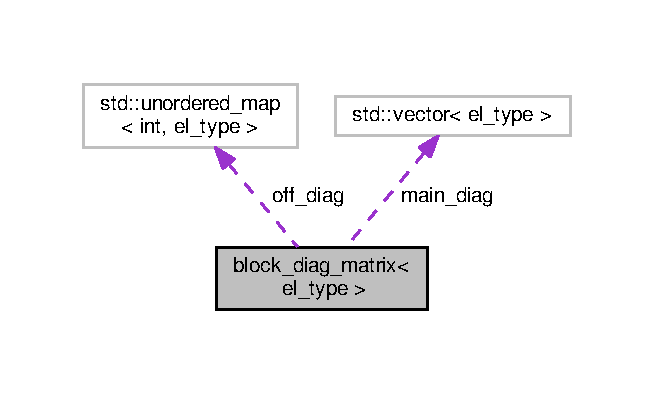
\includegraphics[width=314pt]{classblock__diag__matrix__coll__graph}
\end{center}
\end{figure}
\subsection*{Public Types}
\begin{DoxyCompactItemize}
\item 
typedef std\+::unordered\+\_\+map$<$ int, el\+\_\+type $>$ {\bfseries int\+\_\+elt\+\_\+map}\hypertarget{classblock__diag__matrix_a83f8d88c5e6d2bdaee582cad484cc793}{}\label{classblock__diag__matrix_a83f8d88c5e6d2bdaee582cad484cc793}

\item 
typedef std\+::vector$<$ el\+\_\+type $>$ {\bfseries elt\+\_\+vector\+\_\+type}\hypertarget{classblock__diag__matrix_ab9eac6089c211c3332e3e3acc2c5dd89}{}\label{classblock__diag__matrix_ab9eac6089c211c3332e3e3acc2c5dd89}

\end{DoxyCompactItemize}
\subsection*{Public Member Functions}
\begin{DoxyCompactItemize}
\item 
\hyperlink{classblock__diag__matrix_a1591d461af4469b500f856745ed2d05b}{block\+\_\+diag\+\_\+matrix} (int \hyperlink{classblock__diag__matrix_a7d965a63398622c241a1b28b41cd9d18}{n\+\_\+rows}=0, int \hyperlink{classblock__diag__matrix_a09c9b0481acb773a864fa9f320f76cc7}{n\+\_\+cols}=0)\hypertarget{classblock__diag__matrix_a1591d461af4469b500f856745ed2d05b}{}\label{classblock__diag__matrix_a1591d461af4469b500f856745ed2d05b}

\begin{DoxyCompactList}\small\item\em Constructor for diagonal class. Initializes a 0x0 matrix when given no arguments. \end{DoxyCompactList}\item 
void \hyperlink{classblock__diag__matrix_aa2f3ffb9d4e198ab18262b702c79cadb}{resize} (int n, el\+\_\+type default\+\_\+value)\hypertarget{classblock__diag__matrix_aa2f3ffb9d4e198ab18262b702c79cadb}{}\label{classblock__diag__matrix_aa2f3ffb9d4e198ab18262b702c79cadb}

\begin{DoxyCompactList}\small\item\em Resizes this matrix to an n$\ast$n matrix with default\+\_\+value on the main diagonal. \end{DoxyCompactList}\item 
void \hyperlink{classblock__diag__matrix_a12249531555506377724ff14abec6905}{resize} (int n)\hypertarget{classblock__diag__matrix_a12249531555506377724ff14abec6905}{}\label{classblock__diag__matrix_a12249531555506377724ff14abec6905}

\begin{DoxyCompactList}\small\item\em Resizes this matrix to an n$\ast$n matrix. \end{DoxyCompactList}\item 
int \hyperlink{classblock__diag__matrix_a7d965a63398622c241a1b28b41cd9d18}{n\+\_\+rows} () const 
\item 
int \hyperlink{classblock__diag__matrix_a09c9b0481acb773a864fa9f320f76cc7}{n\+\_\+cols} () const 
\item 
int \hyperlink{classblock__diag__matrix_a7119c39d6ffdf74c2e995d9ae53f57a2}{nnz} () const 
\item 
el\+\_\+type \& \hyperlink{classblock__diag__matrix_a82f0f2e27c91802823c80b1c8007df4d}{operator\mbox{[}$\,$\mbox{]}} (int i)
\item 
el\+\_\+type \& \hyperlink{classblock__diag__matrix_aa57572352da969e948428ad7521a1ce3}{off\+\_\+diagonal} (int i)
\item 
int \hyperlink{classblock__diag__matrix_ad2a00befe5b5c5718e222fa99cbbefd2}{block\+\_\+size} (int i) const 
\item 
void \hyperlink{classblock__diag__matrix_a5f75bcd1cafdb778f2658b7677ad97b9}{sqrt\+\_\+solve} (const elt\+\_\+vector\+\_\+type \&b, elt\+\_\+vector\+\_\+type \&x, bool transposed=false)
\begin{DoxyCompactList}\small\item\em Solves the preconditioned problem $\vert$\+D$\vert$ = Q$\vert$\+V$\vert$Q\textquotesingle{}, where Q\+VQ\textquotesingle{} is the eigendecomposition of D, and $\vert$.$\vert$ is applied elementwise. \end{DoxyCompactList}\item 
void \hyperlink{classblock__diag__matrix_a9cc0b7bc0f96b6688edaef61be790430}{solve} (const elt\+\_\+vector\+\_\+type \&b, elt\+\_\+vector\+\_\+type \&x)
\begin{DoxyCompactList}\small\item\em Solves the system Dx = b. \end{DoxyCompactList}\item 
std\+::string \hyperlink{classblock__diag__matrix_a8aa70dbd0e2c29d814fe5c29701b84cc}{to\+\_\+string} () const 
\item 
bool \hyperlink{classblock__diag__matrix_aa6b66605d7e4af701ec12effaa1f0637}{save} (std\+::string filename) const 
\item 
\hyperlink{classblock__diag__matrix_a060d90add0a7490196fd47f5efb1c818}{$\sim$block\+\_\+diag\+\_\+matrix} ()\hypertarget{classblock__diag__matrix_a060d90add0a7490196fd47f5efb1c818}{}\label{classblock__diag__matrix_a060d90add0a7490196fd47f5efb1c818}

\begin{DoxyCompactList}\small\item\em Generic class destructor. \end{DoxyCompactList}\end{DoxyCompactItemize}
\subsection*{Public Attributes}
\begin{DoxyCompactItemize}
\item 
int \hyperlink{classblock__diag__matrix_a8e55b8cb27c7686a6e62f5e1655723b4}{m\+\_\+n\+\_\+size}\hypertarget{classblock__diag__matrix_a8e55b8cb27c7686a6e62f5e1655723b4}{}\label{classblock__diag__matrix_a8e55b8cb27c7686a6e62f5e1655723b4}

\begin{DoxyCompactList}\small\item\em Dimension of the matrix. \end{DoxyCompactList}\item 
int \hyperlink{classblock__diag__matrix_a13fa6893c7125ff3443e75d3b5f64cd9}{nnz\+\_\+count}\hypertarget{classblock__diag__matrix_a13fa6893c7125ff3443e75d3b5f64cd9}{}\label{classblock__diag__matrix_a13fa6893c7125ff3443e75d3b5f64cd9}

\begin{DoxyCompactList}\small\item\em Number of non-\/zeros in the matrix. \end{DoxyCompactList}\item 
elt\+\_\+vector\+\_\+type \hyperlink{classblock__diag__matrix_a74396564eee4ad30c97b0eab031dda32}{main\+\_\+diag}\hypertarget{classblock__diag__matrix_a74396564eee4ad30c97b0eab031dda32}{}\label{classblock__diag__matrix_a74396564eee4ad30c97b0eab031dda32}

\begin{DoxyCompactList}\small\item\em Stores main diagonal elements. \end{DoxyCompactList}\item 
int\+\_\+elt\+\_\+map \hyperlink{classblock__diag__matrix_a894255ea4928f43a2cae577abc4910d3}{off\+\_\+diag}\hypertarget{classblock__diag__matrix_a894255ea4928f43a2cae577abc4910d3}{}\label{classblock__diag__matrix_a894255ea4928f43a2cae577abc4910d3}

\begin{DoxyCompactList}\small\item\em Stores off-\/diagonal elements of 2x2 pivots. \end{DoxyCompactList}\end{DoxyCompactItemize}
\subsection*{Friends}
\begin{DoxyCompactItemize}
\item 
std\+::ostream \& \hyperlink{classblock__diag__matrix_a17f3419f2a6f824dea494d9ac229c000}{operator$<$$<$} (std\+::ostream \&os, const \hyperlink{classblock__diag__matrix}{block\+\_\+diag\+\_\+matrix} \&D)
\end{DoxyCompactItemize}


\subsection{Detailed Description}
\subsubsection*{template$<$class el\+\_\+type$>$\\*
class block\+\_\+diag\+\_\+matrix$<$ el\+\_\+type $>$}

A quick implementation of a diagonal matrix with 1x1 and 2x2 blocks. 

\subsection{Member Function Documentation}
\index{block\+\_\+diag\+\_\+matrix@{block\+\_\+diag\+\_\+matrix}!block\+\_\+size@{block\+\_\+size}}
\index{block\+\_\+size@{block\+\_\+size}!block\+\_\+diag\+\_\+matrix@{block\+\_\+diag\+\_\+matrix}}
\subsubsection[{\texorpdfstring{block\+\_\+size(int i) const }{block_size(int i) const }}]{\setlength{\rightskip}{0pt plus 5cm}template$<$class el\+\_\+type$>$ int {\bf block\+\_\+diag\+\_\+matrix}$<$ el\+\_\+type $>$\+::block\+\_\+size (
\begin{DoxyParamCaption}
\item[{int}]{i}
\end{DoxyParamCaption}
) const\hspace{0.3cm}{\ttfamily [inline]}}\hypertarget{classblock__diag__matrix_ad2a00befe5b5c5718e222fa99cbbefd2}{}\label{classblock__diag__matrix_ad2a00befe5b5c5718e222fa99cbbefd2}

\begin{DoxyParams}{Parameters}
{\em i} & the index of the element. \\
\hline
\end{DoxyParams}
\begin{DoxyReturn}{Returns}
2 if there is a diagonal pivot at D(i,i) and D(i+1,i+1). -\/2 if there is a diagonal pivot at D(i-\/1,i-\/1) and D(i,i). 1 if the pivot is only a 1x1 block. 
\end{DoxyReturn}
\index{block\+\_\+diag\+\_\+matrix@{block\+\_\+diag\+\_\+matrix}!n\+\_\+cols@{n\+\_\+cols}}
\index{n\+\_\+cols@{n\+\_\+cols}!block\+\_\+diag\+\_\+matrix@{block\+\_\+diag\+\_\+matrix}}
\subsubsection[{\texorpdfstring{n\+\_\+cols() const }{n_cols() const }}]{\setlength{\rightskip}{0pt plus 5cm}template$<$class el\+\_\+type$>$ int {\bf block\+\_\+diag\+\_\+matrix}$<$ el\+\_\+type $>$\+::n\+\_\+cols (
\begin{DoxyParamCaption}
{}
\end{DoxyParamCaption}
) const\hspace{0.3cm}{\ttfamily [inline]}}\hypertarget{classblock__diag__matrix_a09c9b0481acb773a864fa9f320f76cc7}{}\label{classblock__diag__matrix_a09c9b0481acb773a864fa9f320f76cc7}
\begin{DoxyReturn}{Returns}
Number of cols in the matrix. 
\end{DoxyReturn}
\index{block\+\_\+diag\+\_\+matrix@{block\+\_\+diag\+\_\+matrix}!n\+\_\+rows@{n\+\_\+rows}}
\index{n\+\_\+rows@{n\+\_\+rows}!block\+\_\+diag\+\_\+matrix@{block\+\_\+diag\+\_\+matrix}}
\subsubsection[{\texorpdfstring{n\+\_\+rows() const }{n_rows() const }}]{\setlength{\rightskip}{0pt plus 5cm}template$<$class el\+\_\+type$>$ int {\bf block\+\_\+diag\+\_\+matrix}$<$ el\+\_\+type $>$\+::n\+\_\+rows (
\begin{DoxyParamCaption}
{}
\end{DoxyParamCaption}
) const\hspace{0.3cm}{\ttfamily [inline]}}\hypertarget{classblock__diag__matrix_a7d965a63398622c241a1b28b41cd9d18}{}\label{classblock__diag__matrix_a7d965a63398622c241a1b28b41cd9d18}
\begin{DoxyReturn}{Returns}
Number of rows in the matrix. 
\end{DoxyReturn}
\index{block\+\_\+diag\+\_\+matrix@{block\+\_\+diag\+\_\+matrix}!nnz@{nnz}}
\index{nnz@{nnz}!block\+\_\+diag\+\_\+matrix@{block\+\_\+diag\+\_\+matrix}}
\subsubsection[{\texorpdfstring{nnz() const }{nnz() const }}]{\setlength{\rightskip}{0pt plus 5cm}template$<$class el\+\_\+type$>$ int {\bf block\+\_\+diag\+\_\+matrix}$<$ el\+\_\+type $>$\+::nnz (
\begin{DoxyParamCaption}
{}
\end{DoxyParamCaption}
) const\hspace{0.3cm}{\ttfamily [inline]}}\hypertarget{classblock__diag__matrix_a7119c39d6ffdf74c2e995d9ae53f57a2}{}\label{classblock__diag__matrix_a7119c39d6ffdf74c2e995d9ae53f57a2}
\begin{DoxyReturn}{Returns}
Number of nonzeros in the matrix. 
\end{DoxyReturn}
\index{block\+\_\+diag\+\_\+matrix@{block\+\_\+diag\+\_\+matrix}!off\+\_\+diagonal@{off\+\_\+diagonal}}
\index{off\+\_\+diagonal@{off\+\_\+diagonal}!block\+\_\+diag\+\_\+matrix@{block\+\_\+diag\+\_\+matrix}}
\subsubsection[{\texorpdfstring{off\+\_\+diagonal(int i)}{off_diagonal(int i)}}]{\setlength{\rightskip}{0pt plus 5cm}template$<$class el\+\_\+type$>$ el\+\_\+type\& {\bf block\+\_\+diag\+\_\+matrix}$<$ el\+\_\+type $>$\+::off\+\_\+diagonal (
\begin{DoxyParamCaption}
\item[{int}]{i}
\end{DoxyParamCaption}
)\hspace{0.3cm}{\ttfamily [inline]}}\hypertarget{classblock__diag__matrix_aa57572352da969e948428ad7521a1ce3}{}\label{classblock__diag__matrix_aa57572352da969e948428ad7521a1ce3}

\begin{DoxyParams}{Parameters}
{\em i} & the index of the element. \\
\hline
\end{DoxyParams}
\begin{DoxyReturn}{Returns}
The D(i+1,i)th element. 
\end{DoxyReturn}
\index{block\+\_\+diag\+\_\+matrix@{block\+\_\+diag\+\_\+matrix}!operator\mbox{[}$\,$\mbox{]}@{operator[]}}
\index{operator\mbox{[}$\,$\mbox{]}@{operator[]}!block\+\_\+diag\+\_\+matrix@{block\+\_\+diag\+\_\+matrix}}
\subsubsection[{\texorpdfstring{operator[](int i)}{operator[](int i)}}]{\setlength{\rightskip}{0pt plus 5cm}template$<$class el\+\_\+type$>$ el\+\_\+type\& {\bf block\+\_\+diag\+\_\+matrix}$<$ el\+\_\+type $>$\+::operator\mbox{[}$\,$\mbox{]} (
\begin{DoxyParamCaption}
\item[{int}]{i}
\end{DoxyParamCaption}
)\hspace{0.3cm}{\ttfamily [inline]}}\hypertarget{classblock__diag__matrix_a82f0f2e27c91802823c80b1c8007df4d}{}\label{classblock__diag__matrix_a82f0f2e27c91802823c80b1c8007df4d}

\begin{DoxyParams}{Parameters}
{\em i} & the index of the element. \\
\hline
\end{DoxyParams}
\begin{DoxyReturn}{Returns}
The D(i,i)th element. 
\end{DoxyReturn}
\index{block\+\_\+diag\+\_\+matrix@{block\+\_\+diag\+\_\+matrix}!save@{save}}
\index{save@{save}!block\+\_\+diag\+\_\+matrix@{block\+\_\+diag\+\_\+matrix}}
\subsubsection[{\texorpdfstring{save(std\+::string filename) const }{save(std::string filename) const }}]{\setlength{\rightskip}{0pt plus 5cm}template$<$class el\+\_\+type $>$ bool {\bf block\+\_\+diag\+\_\+matrix}$<$ el\+\_\+type $>$\+::save (
\begin{DoxyParamCaption}
\item[{std\+::string}]{filename}
\end{DoxyParamCaption}
) const}\hypertarget{classblock__diag__matrix_aa6b66605d7e4af701ec12effaa1f0637}{}\label{classblock__diag__matrix_aa6b66605d7e4af701ec12effaa1f0637}

\begin{DoxyParams}{Parameters}
{\em filename} & the filename of the matrix to be saved. All matrices saved are in matrix market format (.mtx). \\
\hline
\end{DoxyParams}
\begin{DoxyReturn}{Returns}
True if the save succeeded, false otherwise. 
\end{DoxyReturn}
\index{block\+\_\+diag\+\_\+matrix@{block\+\_\+diag\+\_\+matrix}!solve@{solve}}
\index{solve@{solve}!block\+\_\+diag\+\_\+matrix@{block\+\_\+diag\+\_\+matrix}}
\subsubsection[{\texorpdfstring{solve(const elt\+\_\+vector\+\_\+type \&b, elt\+\_\+vector\+\_\+type \&x)}{solve(const elt_vector_type &b, elt_vector_type &x)}}]{\setlength{\rightskip}{0pt plus 5cm}template$<$class el\+\_\+type$>$ void {\bf block\+\_\+diag\+\_\+matrix}$<$ el\+\_\+type $>$\+::solve (
\begin{DoxyParamCaption}
\item[{const elt\+\_\+vector\+\_\+type \&}]{b, }
\item[{elt\+\_\+vector\+\_\+type \&}]{x}
\end{DoxyParamCaption}
)\hspace{0.3cm}{\ttfamily [inline]}}\hypertarget{classblock__diag__matrix_a9cc0b7bc0f96b6688edaef61be790430}{}\label{classblock__diag__matrix_a9cc0b7bc0f96b6688edaef61be790430}


Solves the system Dx = b. 


\begin{DoxyParams}{Parameters}
{\em b} & the right hand side. \\
\hline
{\em x} & a storage vector for the solution (must be same size as b). \\
\hline
\end{DoxyParams}
\index{block\+\_\+diag\+\_\+matrix@{block\+\_\+diag\+\_\+matrix}!sqrt\+\_\+solve@{sqrt\+\_\+solve}}
\index{sqrt\+\_\+solve@{sqrt\+\_\+solve}!block\+\_\+diag\+\_\+matrix@{block\+\_\+diag\+\_\+matrix}}
\subsubsection[{\texorpdfstring{sqrt\+\_\+solve(const elt\+\_\+vector\+\_\+type \&b, elt\+\_\+vector\+\_\+type \&x, bool transposed=false)}{sqrt_solve(const elt_vector_type &b, elt_vector_type &x, bool transposed=false)}}]{\setlength{\rightskip}{0pt plus 5cm}template$<$class el\+\_\+type$>$ void {\bf block\+\_\+diag\+\_\+matrix}$<$ el\+\_\+type $>$\+::sqrt\+\_\+solve (
\begin{DoxyParamCaption}
\item[{const elt\+\_\+vector\+\_\+type \&}]{b, }
\item[{elt\+\_\+vector\+\_\+type \&}]{x, }
\item[{bool}]{transposed = {\ttfamily false}}
\end{DoxyParamCaption}
)\hspace{0.3cm}{\ttfamily [inline]}}\hypertarget{classblock__diag__matrix_a5f75bcd1cafdb778f2658b7677ad97b9}{}\label{classblock__diag__matrix_a5f75bcd1cafdb778f2658b7677ad97b9}


Solves the preconditioned problem $\vert$\+D$\vert$ = Q$\vert$\+V$\vert$Q\textquotesingle{}, where Q\+VQ\textquotesingle{} is the eigendecomposition of D, and $\vert$.$\vert$ is applied elementwise. 


\begin{DoxyParams}{Parameters}
{\em b} & the right hand side. \\
\hline
{\em x} & a storage vector for the solution (must be same size as b). \\
\hline
{\em transposed} & solves $\vert$\+V$\vert$$^\wedge$(1/2)Q\textquotesingle{} if true, Q$\vert$\+V$\vert$$^\wedge$(1/2) if false. \\
\hline
\end{DoxyParams}
\index{block\+\_\+diag\+\_\+matrix@{block\+\_\+diag\+\_\+matrix}!to\+\_\+string@{to\+\_\+string}}
\index{to\+\_\+string@{to\+\_\+string}!block\+\_\+diag\+\_\+matrix@{block\+\_\+diag\+\_\+matrix}}
\subsubsection[{\texorpdfstring{to\+\_\+string() const }{to_string() const }}]{\setlength{\rightskip}{0pt plus 5cm}template$<$class el\+\_\+type $>$ std\+::string {\bf block\+\_\+diag\+\_\+matrix}$<$ el\+\_\+type $>$\+::to\+\_\+string (
\begin{DoxyParamCaption}
{}
\end{DoxyParamCaption}
) const}\hypertarget{classblock__diag__matrix_a8aa70dbd0e2c29d814fe5c29701b84cc}{}\label{classblock__diag__matrix_a8aa70dbd0e2c29d814fe5c29701b84cc}
\begin{DoxyReturn}{Returns}
A string reprepsentation of this matrix. 
\end{DoxyReturn}


\subsection{Friends And Related Function Documentation}
\index{block\+\_\+diag\+\_\+matrix@{block\+\_\+diag\+\_\+matrix}!operator$<$$<$@{operator$<$$<$}}
\index{operator$<$$<$@{operator$<$$<$}!block\+\_\+diag\+\_\+matrix@{block\+\_\+diag\+\_\+matrix}}
\subsubsection[{\texorpdfstring{operator$<$$<$}{operator<<}}]{\setlength{\rightskip}{0pt plus 5cm}template$<$class el\+\_\+type$>$ std\+::ostream\& operator$<$$<$ (
\begin{DoxyParamCaption}
\item[{std\+::ostream \&}]{os, }
\item[{const {\bf block\+\_\+diag\+\_\+matrix}$<$ el\+\_\+type $>$ \&}]{D}
\end{DoxyParamCaption}
)\hspace{0.3cm}{\ttfamily [friend]}}\hypertarget{classblock__diag__matrix_a17f3419f2a6f824dea494d9ac229c000}{}\label{classblock__diag__matrix_a17f3419f2a6f824dea494d9ac229c000}
Allows outputting the contents of the matrix via $<$$<$ operators. 

The documentation for this class was generated from the following files\+:\begin{DoxyCompactItemize}
\item 
source/block\+\_\+diag\+\_\+matrix.\+h\item 
source/block\+\_\+diag\+\_\+matrix\+\_\+save.\+h\item 
source/block\+\_\+diag\+\_\+matrix\+\_\+to\+\_\+string.\+h\end{DoxyCompactItemize}

\hypertarget{structsymildl_1_1equilibration__type}{}\section{symildl\+:\+:equilibration\+\_\+type Struct Reference}
\label{structsymildl_1_1equilibration__type}\index{symildl\+::equilibration\+\_\+type@{symildl\+::equilibration\+\_\+type}}
\subsection*{Public Types}
\begin{DoxyCompactItemize}
\item 
enum \{ {\bfseries N\+O\+NE}, 
{\bfseries B\+U\+N\+CH}, 
{\bfseries R\+U\+IZ}, 
{\bfseries M\+C64}
 \}\hypertarget{structsymildl_1_1equilibration__type_ab010e95fc085b7e5d53fa0a78ac40cb9}{}\label{structsymildl_1_1equilibration__type_ab010e95fc085b7e5d53fa0a78ac40cb9}

\end{DoxyCompactItemize}


The documentation for this struct was generated from the following file\+:\begin{DoxyCompactItemize}
\item 
source/solver.\+h\end{DoxyCompactItemize}

\hypertarget{classlil__sparse__matrix}{}\section{lil\+\_\+sparse\+\_\+matrix$<$ el\+\_\+type $>$ Class Template Reference}
\label{classlil__sparse__matrix}\index{lil\+\_\+sparse\+\_\+matrix$<$ el\+\_\+type $>$@{lil\+\_\+sparse\+\_\+matrix$<$ el\+\_\+type $>$}}


The abstract parent of all sparse matrices.  




{\ttfamily \#include $<$lil\+\_\+sparse\+\_\+matrix.\+h$>$}



Inheritance diagram for lil\+\_\+sparse\+\_\+matrix$<$ el\+\_\+type $>$\+:\nopagebreak
\begin{figure}[H]
\begin{center}
\leavevmode
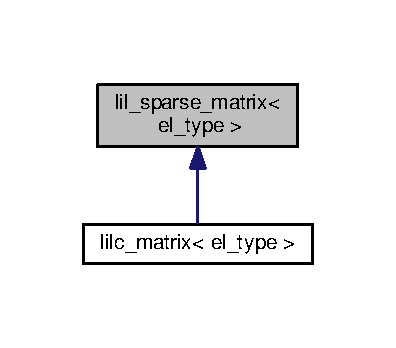
\includegraphics[width=190pt]{classlil__sparse__matrix__inherit__graph}
\end{center}
\end{figure}


Collaboration diagram for lil\+\_\+sparse\+\_\+matrix$<$ el\+\_\+type $>$\+:\nopagebreak
\begin{figure}[H]
\begin{center}
\leavevmode
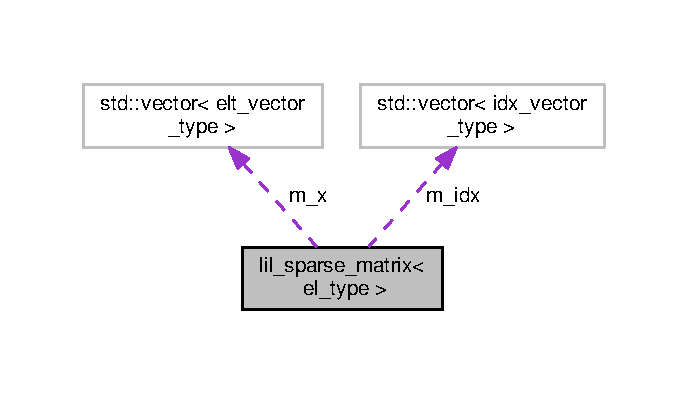
\includegraphics[width=330pt]{classlil__sparse__matrix__coll__graph}
\end{center}
\end{figure}
\subsection*{Public Types}
\begin{DoxyCompactItemize}
\item 
typedef vector$<$ int $>$ {\bfseries idx\+\_\+vector\+\_\+type}\hypertarget{classlil__sparse__matrix_aac6d12fd87c19ad7d39f0fbdf7e0aa01}{}\label{classlil__sparse__matrix_aac6d12fd87c19ad7d39f0fbdf7e0aa01}

\item 
typedef vector$<$ el\+\_\+type $>$ {\bfseries elt\+\_\+vector\+\_\+type}\hypertarget{classlil__sparse__matrix_aac442ebc44706f184c7ce4ee7e1fdd6d}{}\label{classlil__sparse__matrix_aac442ebc44706f184c7ce4ee7e1fdd6d}

\end{DoxyCompactItemize}
\subsection*{Public Member Functions}
\begin{DoxyCompactItemize}
\item 
\hyperlink{classlil__sparse__matrix_a74dff1c9df79556341d714d4530ffe38}{lil\+\_\+sparse\+\_\+matrix} (int \hyperlink{classlil__sparse__matrix_a29e9ea5f7c8a9fca9029a91b39c592e0}{n\+\_\+rows}, int \hyperlink{classlil__sparse__matrix_ac88631204bcf7c9a223fb082a7d0cd3d}{n\+\_\+cols})\hypertarget{classlil__sparse__matrix_a74dff1c9df79556341d714d4530ffe38}{}\label{classlil__sparse__matrix_a74dff1c9df79556341d714d4530ffe38}

\begin{DoxyCompactList}\small\item\em Default constructor for an abstract matrix. This constructor will be extended by base classes depending on the representation of the matrix (L\+I\+L-\/C or L\+I\+L-\/R). \end{DoxyCompactList}\item 
int \hyperlink{classlil__sparse__matrix_a29e9ea5f7c8a9fca9029a91b39c592e0}{n\+\_\+rows} () const 
\item 
int \hyperlink{classlil__sparse__matrix_ac88631204bcf7c9a223fb082a7d0cd3d}{n\+\_\+cols} () const 
\item 
int \hyperlink{classlil__sparse__matrix_a40bc09d3b6716e57134eed0aeba49199}{nnz} () const 
\item 
virtual el\+\_\+type \hyperlink{classlil__sparse__matrix_a03af482b9f3d8c8b522dd5e49a2500ee}{coeff} (const int \&i, const int \&j, int offset=0) const =0
\begin{DoxyCompactList}\small\item\em Returns A\+\_\+ij (zero-\/indexed). This function should be extended by subclasses as it is dependent on the matrix storage type. \end{DoxyCompactList}\item 
virtual std\+::string \hyperlink{classlil__sparse__matrix_a5c2c43867660473176de5c73ebdac7be}{to\+\_\+string} () const =0
\item 
virtual \hyperlink{classlil__sparse__matrix_aebd4e61eeb73f709d0900cc064d8986d}{$\sim$lil\+\_\+sparse\+\_\+matrix} ()
\end{DoxyCompactItemize}
\subsection*{Public Attributes}
\begin{DoxyCompactItemize}
\item 
int \hyperlink{classlil__sparse__matrix_a6eac075dab519f837ae660c9ef933eb9}{m\+\_\+n\+\_\+rows}\hypertarget{classlil__sparse__matrix_a6eac075dab519f837ae660c9ef933eb9}{}\label{classlil__sparse__matrix_a6eac075dab519f837ae660c9ef933eb9}

\begin{DoxyCompactList}\small\item\em Number of rows in the matrix. \end{DoxyCompactList}\item 
int \hyperlink{classlil__sparse__matrix_aab335a46ece471fd0edf52540e24225a}{m\+\_\+n\+\_\+cols}\hypertarget{classlil__sparse__matrix_aab335a46ece471fd0edf52540e24225a}{}\label{classlil__sparse__matrix_aab335a46ece471fd0edf52540e24225a}

\begin{DoxyCompactList}\small\item\em Number of cols in the matrix. \end{DoxyCompactList}\item 
int \hyperlink{classlil__sparse__matrix_acdc8477f4f3893490bbf0b196438fab8}{nnz\+\_\+count}\hypertarget{classlil__sparse__matrix_acdc8477f4f3893490bbf0b196438fab8}{}\label{classlil__sparse__matrix_acdc8477f4f3893490bbf0b196438fab8}

\begin{DoxyCompactList}\small\item\em Number of nonzeros in the matrix. \end{DoxyCompactList}\item 
el\+\_\+type \hyperlink{classlil__sparse__matrix_af764d0312eb9f7939ab144b12972bf56}{eps}\hypertarget{classlil__sparse__matrix_af764d0312eb9f7939ab144b12972bf56}{}\label{classlil__sparse__matrix_af764d0312eb9f7939ab144b12972bf56}

\begin{DoxyCompactList}\small\item\em Machine epsilon for el\+\_\+type. \end{DoxyCompactList}\item 
vector$<$ idx\+\_\+vector\+\_\+type $>$ \hyperlink{classlil__sparse__matrix_a133b6db4ddc63626a8787abbb2564aa6}{m\+\_\+idx}\hypertarget{classlil__sparse__matrix_a133b6db4ddc63626a8787abbb2564aa6}{}\label{classlil__sparse__matrix_a133b6db4ddc63626a8787abbb2564aa6}

\begin{DoxyCompactList}\small\item\em The row/col indices. The way m\+\_\+idx is used depends on whether the matrix is in L\+I\+L-\/C or L\+I\+L-\/R. \end{DoxyCompactList}\item 
vector$<$ elt\+\_\+vector\+\_\+type $>$ \hyperlink{classlil__sparse__matrix_ac2abac5da68172e1e3e21376247643de}{m\+\_\+x}\hypertarget{classlil__sparse__matrix_ac2abac5da68172e1e3e21376247643de}{}\label{classlil__sparse__matrix_ac2abac5da68172e1e3e21376247643de}

\begin{DoxyCompactList}\small\item\em The values of the nonzeros in the matrix. \end{DoxyCompactList}\end{DoxyCompactItemize}
\subsection*{Friends}
\begin{DoxyCompactItemize}
\item 
std\+::ostream \& \hyperlink{classlil__sparse__matrix_a9f5c4b354ab1ce7fd0bf6bb146b1f3c0}{operator$<$$<$} (std\+::ostream \&os, const \hyperlink{classlil__sparse__matrix}{lil\+\_\+sparse\+\_\+matrix} \&A)\hypertarget{classlil__sparse__matrix_a9f5c4b354ab1ce7fd0bf6bb146b1f3c0}{}\label{classlil__sparse__matrix_a9f5c4b354ab1ce7fd0bf6bb146b1f3c0}

\begin{DoxyCompactList}\small\item\em Allows outputting the contents of the matrix via $<$$<$ operators. \end{DoxyCompactList}\end{DoxyCompactItemize}


\subsection{Detailed Description}
\subsubsection*{template$<$class el\+\_\+type$>$\\*
class lil\+\_\+sparse\+\_\+matrix$<$ el\+\_\+type $>$}

The abstract parent of all sparse matrices. 

\subsection{Constructor \& Destructor Documentation}
\index{lil\+\_\+sparse\+\_\+matrix@{lil\+\_\+sparse\+\_\+matrix}!````~lil\+\_\+sparse\+\_\+matrix@{$\sim$lil\+\_\+sparse\+\_\+matrix}}
\index{````~lil\+\_\+sparse\+\_\+matrix@{$\sim$lil\+\_\+sparse\+\_\+matrix}!lil\+\_\+sparse\+\_\+matrix@{lil\+\_\+sparse\+\_\+matrix}}
\subsubsection[{\texorpdfstring{$\sim$lil\+\_\+sparse\+\_\+matrix()}{~lil_sparse_matrix()}}]{\setlength{\rightskip}{0pt plus 5cm}template$<$class el\+\_\+type $>$ virtual {\bf lil\+\_\+sparse\+\_\+matrix}$<$ el\+\_\+type $>$\+::$\sim${\bf lil\+\_\+sparse\+\_\+matrix} (
\begin{DoxyParamCaption}
{}
\end{DoxyParamCaption}
)\hspace{0.3cm}{\ttfamily [inline]}, {\ttfamily [virtual]}}\hypertarget{classlil__sparse__matrix_aebd4e61eeb73f709d0900cc064d8986d}{}\label{classlil__sparse__matrix_aebd4e61eeb73f709d0900cc064d8986d}
Generic class destructor. 

\subsection{Member Function Documentation}
\index{lil\+\_\+sparse\+\_\+matrix@{lil\+\_\+sparse\+\_\+matrix}!coeff@{coeff}}
\index{coeff@{coeff}!lil\+\_\+sparse\+\_\+matrix@{lil\+\_\+sparse\+\_\+matrix}}
\subsubsection[{\texorpdfstring{coeff(const int \&i, const int \&j, int offset=0) const =0}{coeff(const int &i, const int &j, int offset=0) const =0}}]{\setlength{\rightskip}{0pt plus 5cm}template$<$class el\+\_\+type $>$ virtual el\+\_\+type {\bf lil\+\_\+sparse\+\_\+matrix}$<$ el\+\_\+type $>$\+::coeff (
\begin{DoxyParamCaption}
\item[{const int \&}]{i, }
\item[{const int \&}]{j, }
\item[{int}]{offset = {\ttfamily 0}}
\end{DoxyParamCaption}
) const\hspace{0.3cm}{\ttfamily [pure virtual]}}\hypertarget{classlil__sparse__matrix_a03af482b9f3d8c8b522dd5e49a2500ee}{}\label{classlil__sparse__matrix_a03af482b9f3d8c8b522dd5e49a2500ee}


Returns A\+\_\+ij (zero-\/indexed). This function should be extended by subclasses as it is dependent on the matrix storage type. 


\begin{DoxyParams}{Parameters}
{\em i} & the row of the (i,j)th element (zero-\/indexed). \\
\hline
{\em j} & the col of the (i,j)th element (zero-\/indexed). \\
\hline
{\em offset} & an optional search offset for use in linear search (start at offset instead of 0). \\
\hline
\end{DoxyParams}
\begin{DoxyReturn}{Returns}
The (i,j)th element of the matrix. 
\end{DoxyReturn}


Implemented in \hyperlink{classlilc__matrix_a0e59d373ec514c8cb264da653d36f753}{lilc\+\_\+matrix$<$ el\+\_\+type $>$}.

\index{lil\+\_\+sparse\+\_\+matrix@{lil\+\_\+sparse\+\_\+matrix}!n\+\_\+cols@{n\+\_\+cols}}
\index{n\+\_\+cols@{n\+\_\+cols}!lil\+\_\+sparse\+\_\+matrix@{lil\+\_\+sparse\+\_\+matrix}}
\subsubsection[{\texorpdfstring{n\+\_\+cols() const }{n_cols() const }}]{\setlength{\rightskip}{0pt plus 5cm}template$<$class el\+\_\+type $>$ int {\bf lil\+\_\+sparse\+\_\+matrix}$<$ el\+\_\+type $>$\+::n\+\_\+cols (
\begin{DoxyParamCaption}
{}
\end{DoxyParamCaption}
) const\hspace{0.3cm}{\ttfamily [inline]}}\hypertarget{classlil__sparse__matrix_ac88631204bcf7c9a223fb082a7d0cd3d}{}\label{classlil__sparse__matrix_ac88631204bcf7c9a223fb082a7d0cd3d}
\begin{DoxyReturn}{Returns}
Number of cols in the matrix. 
\end{DoxyReturn}
\index{lil\+\_\+sparse\+\_\+matrix@{lil\+\_\+sparse\+\_\+matrix}!n\+\_\+rows@{n\+\_\+rows}}
\index{n\+\_\+rows@{n\+\_\+rows}!lil\+\_\+sparse\+\_\+matrix@{lil\+\_\+sparse\+\_\+matrix}}
\subsubsection[{\texorpdfstring{n\+\_\+rows() const }{n_rows() const }}]{\setlength{\rightskip}{0pt plus 5cm}template$<$class el\+\_\+type $>$ int {\bf lil\+\_\+sparse\+\_\+matrix}$<$ el\+\_\+type $>$\+::n\+\_\+rows (
\begin{DoxyParamCaption}
{}
\end{DoxyParamCaption}
) const\hspace{0.3cm}{\ttfamily [inline]}}\hypertarget{classlil__sparse__matrix_a29e9ea5f7c8a9fca9029a91b39c592e0}{}\label{classlil__sparse__matrix_a29e9ea5f7c8a9fca9029a91b39c592e0}
\begin{DoxyReturn}{Returns}
Number of rows in the matrix. 
\end{DoxyReturn}
\index{lil\+\_\+sparse\+\_\+matrix@{lil\+\_\+sparse\+\_\+matrix}!nnz@{nnz}}
\index{nnz@{nnz}!lil\+\_\+sparse\+\_\+matrix@{lil\+\_\+sparse\+\_\+matrix}}
\subsubsection[{\texorpdfstring{nnz() const }{nnz() const }}]{\setlength{\rightskip}{0pt plus 5cm}template$<$class el\+\_\+type $>$ int {\bf lil\+\_\+sparse\+\_\+matrix}$<$ el\+\_\+type $>$\+::nnz (
\begin{DoxyParamCaption}
{}
\end{DoxyParamCaption}
) const\hspace{0.3cm}{\ttfamily [inline]}}\hypertarget{classlil__sparse__matrix_a40bc09d3b6716e57134eed0aeba49199}{}\label{classlil__sparse__matrix_a40bc09d3b6716e57134eed0aeba49199}
\begin{DoxyReturn}{Returns}
Number of nonzeros in the matrix. 
\end{DoxyReturn}
\index{lil\+\_\+sparse\+\_\+matrix@{lil\+\_\+sparse\+\_\+matrix}!to\+\_\+string@{to\+\_\+string}}
\index{to\+\_\+string@{to\+\_\+string}!lil\+\_\+sparse\+\_\+matrix@{lil\+\_\+sparse\+\_\+matrix}}
\subsubsection[{\texorpdfstring{to\+\_\+string() const =0}{to_string() const =0}}]{\setlength{\rightskip}{0pt plus 5cm}template$<$class el\+\_\+type $>$ virtual std\+::string {\bf lil\+\_\+sparse\+\_\+matrix}$<$ el\+\_\+type $>$\+::to\+\_\+string (
\begin{DoxyParamCaption}
{}
\end{DoxyParamCaption}
) const\hspace{0.3cm}{\ttfamily [pure virtual]}}\hypertarget{classlil__sparse__matrix_a5c2c43867660473176de5c73ebdac7be}{}\label{classlil__sparse__matrix_a5c2c43867660473176de5c73ebdac7be}
\begin{DoxyReturn}{Returns}
A string reprepsentation of this matrix. 
\end{DoxyReturn}


Implemented in \hyperlink{classlilc__matrix_a60c5a4a0ec9a49d43be087b6d67f4df2}{lilc\+\_\+matrix$<$ el\+\_\+type $>$}.



The documentation for this class was generated from the following file\+:\begin{DoxyCompactItemize}
\item 
source/lil\+\_\+sparse\+\_\+matrix.\+h\end{DoxyCompactItemize}

\hypertarget{classlilc__matrix}{}\section{lilc\+\_\+matrix$<$ el\+\_\+type $>$ Class Template Reference}
\label{classlilc__matrix}\index{lilc\+\_\+matrix$<$ el\+\_\+type $>$@{lilc\+\_\+matrix$<$ el\+\_\+type $>$}}


A list-\/of-\/lists (L\+IL) matrix in column oriented format.  




{\ttfamily \#include $<$lilc\+\_\+matrix\+\_\+declarations.\+h$>$}



Inheritance diagram for lilc\+\_\+matrix$<$ el\+\_\+type $>$\+:\nopagebreak
\begin{figure}[H]
\begin{center}
\leavevmode
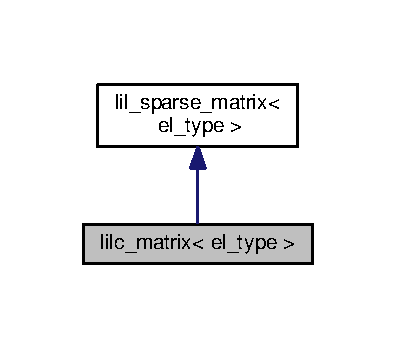
\includegraphics[width=190pt]{classlilc__matrix__inherit__graph}
\end{center}
\end{figure}


Collaboration diagram for lilc\+\_\+matrix$<$ el\+\_\+type $>$\+:\nopagebreak
\begin{figure}[H]
\begin{center}
\leavevmode
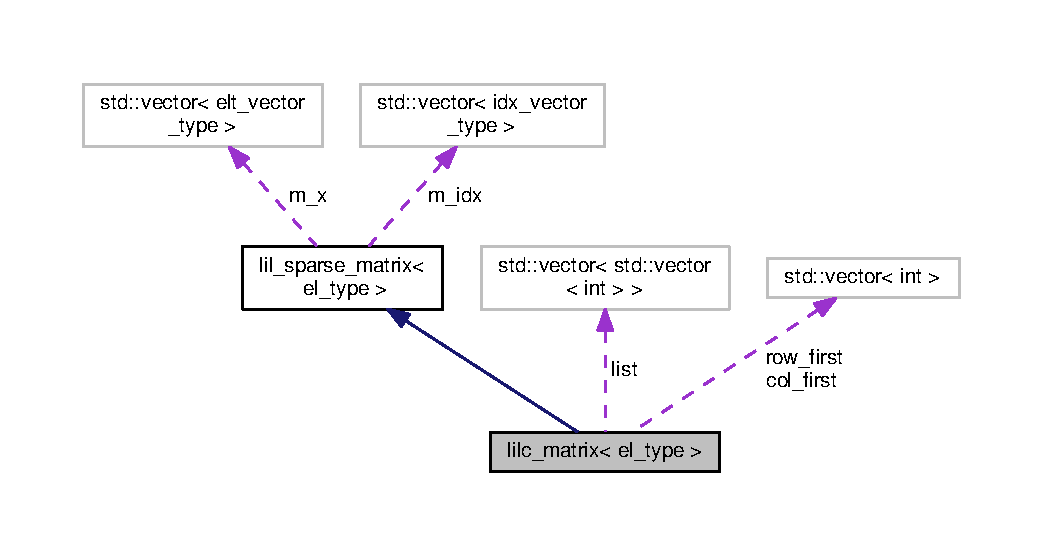
\includegraphics[width=350pt]{classlilc__matrix__coll__graph}
\end{center}
\end{figure}
\subsection*{Classes}
\begin{DoxyCompactItemize}
\item 
struct \hyperlink{structlilc__matrix_1_1pivot__type}{pivot\+\_\+type}
\end{DoxyCompactItemize}
\subsection*{Public Types}
\begin{DoxyCompactItemize}
\item 
typedef \hyperlink{classlil__sparse__matrix}{lil\+\_\+sparse\+\_\+matrix}$<$ el\+\_\+type $>$\+::idx\+\_\+vector\+\_\+type {\bfseries idx\+\_\+vector\+\_\+type}\hypertarget{classlilc__matrix_a83c70482c28275881562ee3937b5f591}{}\label{classlilc__matrix_a83c70482c28275881562ee3937b5f591}

\item 
typedef \hyperlink{classlil__sparse__matrix}{lil\+\_\+sparse\+\_\+matrix}$<$ el\+\_\+type $>$\+::elt\+\_\+vector\+\_\+type {\bfseries elt\+\_\+vector\+\_\+type}\hypertarget{classlilc__matrix_aa5a7b6e31a6c9ebf2ea3a898fe646af6}{}\label{classlilc__matrix_aa5a7b6e31a6c9ebf2ea3a898fe646af6}

\item 
typedef idx\+\_\+vector\+\_\+type\+::iterator {\bfseries idx\+\_\+it}\hypertarget{classlilc__matrix_a8cd399b5bc0ef50dcf5a59a671e32248}{}\label{classlilc__matrix_a8cd399b5bc0ef50dcf5a59a671e32248}

\item 
typedef elt\+\_\+vector\+\_\+type\+::iterator {\bfseries elt\+\_\+it}\hypertarget{classlilc__matrix_ad34c37b7095e283a7e5d7160fe26fd1b}{}\label{classlilc__matrix_ad34c37b7095e283a7e5d7160fe26fd1b}

\end{DoxyCompactItemize}
\subsection*{Public Member Functions}
\begin{DoxyCompactItemize}
\item 
\hyperlink{classlilc__matrix_acdaad0931ff27d7bfc361d3033713914}{lilc\+\_\+matrix} (int \hyperlink{classlil__sparse__matrix_a29e9ea5f7c8a9fca9029a91b39c592e0}{n\+\_\+rows}=0, int \hyperlink{classlil__sparse__matrix_ac88631204bcf7c9a223fb082a7d0cd3d}{n\+\_\+cols}=0)\hypertarget{classlilc__matrix_acdaad0931ff27d7bfc361d3033713914}{}\label{classlilc__matrix_acdaad0931ff27d7bfc361d3033713914}

\begin{DoxyCompactList}\small\item\em Constructor for a column oriented list-\/of-\/lists (L\+IL) matrix. Space for both the values list and the indices list of the matrix is allocated here. \end{DoxyCompactList}\item 
virtual el\+\_\+type \hyperlink{classlilc__matrix_a0e59d373ec514c8cb264da653d36f753}{coeff} (const int \&i, const int \&j, int offset=0) const 
\begin{DoxyCompactList}\small\item\em Finds the (i,j)th coefficient of the matrix. \end{DoxyCompactList}\item 
bool \hyperlink{classlilc__matrix_a327c165f0c90cd362dd14fc6421ebadd}{coeff\+Ref} (const int \&i, const int \&j, std\+::pair$<$ idx\+\_\+it, elt\+\_\+it $>$ \&its)
\begin{DoxyCompactList}\small\item\em Finds the index/value pointers to (i,j)th coefficient of the matrix. \end{DoxyCompactList}\item 
void \hyperlink{classlilc__matrix_aca815e0ac073abb1e6ef888b09f9e795}{resize} (int \hyperlink{classlil__sparse__matrix_a29e9ea5f7c8a9fca9029a91b39c592e0}{n\+\_\+rows}, int \hyperlink{classlil__sparse__matrix_ac88631204bcf7c9a223fb082a7d0cd3d}{n\+\_\+cols})
\begin{DoxyCompactList}\small\item\em Resizes the matrix. For use in preallocating space before factorization begins. \end{DoxyCompactList}\item 
void \hyperlink{classlilc__matrix_a46161695c5bfb0f43a7dedb9b9146fef}{find\+\_\+root} (int \&s)
\begin{DoxyCompactList}\small\item\em Returns a pseudo-\/peripheral root of A. This is essentially many chained breadth-\/first searchs across the graph of A (where A is viewed as an adjacency matrix). \end{DoxyCompactList}\item 
bool \hyperlink{classlilc__matrix_ad343cd9b2f435f40a9866de050f63ce5}{find\+\_\+level\+\_\+set} (vector$<$ int $>$ \&lvl\+\_\+set, vector$<$ bool $>$ \&visited)
\begin{DoxyCompactList}\small\item\em Returns the next level set given the current level set of A. This is essentially all neighbours of the currently enqueued nodes in breath-\/first search. \end{DoxyCompactList}\item 
void \hyperlink{classlilc__matrix_ab34914d2b48a5bf14e7ef22e89d2f2e7}{sym\+\_\+rcm} (vector$<$ int $>$ \&perm)
\begin{DoxyCompactList}\small\item\em Returns a Reverse Cuthill-\/\+Mc\+Kee ordering of the matrix A (stored in perm). \end{DoxyCompactList}\item 
void \hyperlink{classlilc__matrix_add59bf538bd6b36c7d42ec879bad4da8}{sym\+\_\+amd} (vector$<$ int $>$ \&perm)
\begin{DoxyCompactList}\small\item\em Returns a Approximate Minimum Degree ordering of the matrix A (stored in perm). \end{DoxyCompactList}\item 
void \hyperlink{classlilc__matrix_af72f55f6880cef04205eb3df7018bce9}{sym\+\_\+perm} (vector$<$ int $>$ \&perm)
\begin{DoxyCompactList}\small\item\em Given a permutation vector perm, A is permuted to P\textquotesingle{}AP, where P is the permutation matrix associated with perm. \end{DoxyCompactList}\item 
void \hyperlink{classlilc__matrix_a37fc8dcc40799dfde0decaaf8bd74b51}{sym\+\_\+equil} ()
\begin{DoxyCompactList}\small\item\em The symmetric matrix A is equilibrated and the symmetric equilibrated matrix S\+AS is stored in A, where S is a diagonal scaling matrix. \end{DoxyCompactList}\item 
void \hyperlink{classlilc__matrix_ab5886c7d465252b8d8981d484b51ab58}{ildl} (\hyperlink{classlilc__matrix}{lilc\+\_\+matrix}$<$ el\+\_\+type $>$ \&L, \hyperlink{classblock__diag__matrix}{block\+\_\+diag\+\_\+matrix}$<$ el\+\_\+type $>$ \&D, idx\+\_\+vector\+\_\+type \&perm, const double \&fill\+\_\+factor, const double \&tol, const double \&pp\+\_\+tol, int piv\+\_\+type=pivot\+\_\+type\+::\+B\+KP)
\begin{DoxyCompactList}\small\item\em Performs an L\+DL\textquotesingle{} factorization of this matrix. \end{DoxyCompactList}\item 
void \hyperlink{classlilc__matrix_aefd39d93fc0df6618f7a59a05661c63e}{ildl\+\_\+inplace} (\hyperlink{classblock__diag__matrix}{block\+\_\+diag\+\_\+matrix}$<$ el\+\_\+type $>$ \&D, idx\+\_\+vector\+\_\+type \&perm, const double \&fill\+\_\+factor, const double \&tol, const double \&pp\+\_\+tol, int piv\+\_\+type=pivot\+\_\+type\+::\+B\+KP)
\begin{DoxyCompactList}\small\item\em Performs an {\itshape inplace} L\+DL\textquotesingle{} factorization of this matrix. \end{DoxyCompactList}\item 
void \hyperlink{classlilc__matrix_a9e0dbfcd1cda4ab3bc067b16f17f7f2f}{backsolve} (const elt\+\_\+vector\+\_\+type \&b, elt\+\_\+vector\+\_\+type \&x)
\begin{DoxyCompactList}\small\item\em Performs a back solve of this matrix, assuming that it is lower triangular (stored column major). \end{DoxyCompactList}\item 
void \hyperlink{classlilc__matrix_afd669063a9594f4d33b01f24bf693edd}{forwardsolve} (const elt\+\_\+vector\+\_\+type \&b, elt\+\_\+vector\+\_\+type \&x)
\begin{DoxyCompactList}\small\item\em Performs a forward solve of this matrix, assuming that it is upper triangular (stored row major). \end{DoxyCompactList}\item 
void \hyperlink{classlilc__matrix_a00362a639b1e8ec341014c39afaf5e5a}{multiply} (const elt\+\_\+vector\+\_\+type \&x, elt\+\_\+vector\+\_\+type \&y, bool full\+\_\+mult=true)
\begin{DoxyCompactList}\small\item\em Performs a matrix-\/vector product with this matrix. \end{DoxyCompactList}\item 
void \hyperlink{classlilc__matrix_a0bb81dfe0808df725cf91f0d7639dcd0}{pivot} (\hyperlink{classswap__struct}{swap\+\_\+struct}$<$ el\+\_\+type $>$ \&s, vector$<$ bool $>$ \&in\+\_\+set, \hyperlink{classlilc__matrix}{lilc\+\_\+matrix}$<$ el\+\_\+type $>$ \&L, const int \&k, const int \&r)
\begin{DoxyCompactList}\small\item\em Performs a symmetric permutation between row/col k \& r of A. \end{DoxyCompactList}\item 
void \hyperlink{classlilc__matrix_aaecb203a3a6ebc85bf0c3a603e6b0fa2}{pivotA} (\hyperlink{classswap__struct}{swap\+\_\+struct}$<$ el\+\_\+type $>$ \&s, vector$<$ bool $>$ \&in\+\_\+set, const int \&k, const int \&r)
\begin{DoxyCompactList}\small\item\em The inplace version of the function above. \end{DoxyCompactList}\item 
{\footnotesize template$<$class Container $>$ }\\void \hyperlink{classlilc__matrix_aa1d3045545357a8f33955a87dc55f3aa}{ensure\+\_\+invariant} (const int \&j, const int \&k, Container \&con, bool update\+\_\+list=false)
\begin{DoxyCompactList}\small\item\em Ensures two the invariants observed by A.\+first and A.\+list are held. \end{DoxyCompactList}\item 
void \hyperlink{classlilc__matrix_a177dde39764c88fe4e82b050a5e60303}{advance\+\_\+first} (const int \&k)
\begin{DoxyCompactList}\small\item\em Updates A.\+first for iteration k. \end{DoxyCompactList}\item 
void \hyperlink{classlilc__matrix_ab9ee09328b84657630f52631ea8e5eb1}{advance\+\_\+list} (const int \&k)
\begin{DoxyCompactList}\small\item\em Updates A.\+list for iteration k. \end{DoxyCompactList}\item 
std\+::string \hyperlink{classlilc__matrix_a60c5a4a0ec9a49d43be087b6d67f4df2}{to\+\_\+string} () const 
\begin{DoxyCompactList}\small\item\em Returns a string representation of A, with each column and its corresponding indices \& non-\/zero values printed. \end{DoxyCompactList}\item 
bool \hyperlink{classlilc__matrix_aea5613e9a57231a6991dcf99d6d7b37a}{load} (std\+::string filename)
\begin{DoxyCompactList}\small\item\em Loads a matrix in matrix market format. \end{DoxyCompactList}\item 
bool \hyperlink{classlilc__matrix_ab469044e7f8716bc0dc4f5532e5c756a}{load} (const std\+::vector$<$ int $>$ \&ptr, const std\+::vector$<$ int $>$ \&row, const std\+::vector$<$ el\+\_\+type $>$ \&val)
\begin{DoxyCompactList}\small\item\em Loads a matrix in C\+SC format. \end{DoxyCompactList}\item 
bool \hyperlink{classlilc__matrix_a141bb846350ac12640901f50cffcf529}{load} (const int $\ast$ptr, const int $\ast$row, const el\+\_\+type $\ast$val, int dim)
\begin{DoxyCompactList}\small\item\em Loads a matrix in C\+SC format. Does no error checking on the input vectors. \end{DoxyCompactList}\item 
bool \hyperlink{classlilc__matrix_a2b0161d36019e1abac41b6119b8fa288}{save} (std\+::string filename, bool sym=false)
\begin{DoxyCompactList}\small\item\em Saves a matrix in matrix market format. \end{DoxyCompactList}\end{DoxyCompactItemize}
\subsection*{Public Attributes}
\begin{DoxyCompactItemize}
\item 
std\+::vector$<$ std\+::vector$<$ int $>$ $>$ \hyperlink{classlilc__matrix_ad942a0e5503a2b4327a12287432fca81}{list}\hypertarget{classlilc__matrix_ad942a0e5503a2b4327a12287432fca81}{}\label{classlilc__matrix_ad942a0e5503a2b4327a12287432fca81}

\begin{DoxyCompactList}\small\item\em A list of linked lists that gives the non-\/zero elements in each row of A. Since at any time we may swap between two rows, we require linked lists for each row of A. \end{DoxyCompactList}\item 
std\+::vector$<$ int $>$ \hyperlink{classlilc__matrix_a2ca57e0c3866ed0cf1f17f6253666ebb}{row\+\_\+first}\hypertarget{classlilc__matrix_a2ca57e0c3866ed0cf1f17f6253666ebb}{}\label{classlilc__matrix_a2ca57e0c3866ed0cf1f17f6253666ebb}

\begin{DoxyCompactList}\small\item\em On iteration k, first\mbox{[}i\mbox{]} gives the number of non-\/zero elements on row i of A before A(i, k). \end{DoxyCompactList}\item 
std\+::vector$<$ int $>$ \hyperlink{classlilc__matrix_a36c12de6fccae4ac5a885e8aa60788e9}{col\+\_\+first}\hypertarget{classlilc__matrix_a36c12de6fccae4ac5a885e8aa60788e9}{}\label{classlilc__matrix_a36c12de6fccae4ac5a885e8aa60788e9}

\begin{DoxyCompactList}\small\item\em On iteration k, first\mbox{[}i\mbox{]} gives the number of non-\/zero elements on col i of A before A(i, k). \end{DoxyCompactList}\item 
\hyperlink{classblock__diag__matrix}{block\+\_\+diag\+\_\+matrix}$<$ el\+\_\+type $>$ \hyperlink{classlilc__matrix_afc4659265addfeab376ffaa8f54ed596}{S}\hypertarget{classlilc__matrix_afc4659265addfeab376ffaa8f54ed596}{}\label{classlilc__matrix_afc4659265addfeab376ffaa8f54ed596}

\begin{DoxyCompactList}\small\item\em A diagonal scaling matrix S such that S\+AS will be equilibriated in the max-\/norm (i.\+e. every row/column has norm 1). S is constructed after running the \hyperlink{classlilc__matrix_a37fc8dcc40799dfde0decaaf8bd74b51}{sym\+\_\+equil()} function, after which S\+AS will be stored in place of A. \end{DoxyCompactList}\end{DoxyCompactItemize}


\subsection{Detailed Description}
\subsubsection*{template$<$class el\+\_\+type$>$\\*
class lilc\+\_\+matrix$<$ el\+\_\+type $>$}

A list-\/of-\/lists (L\+IL) matrix in column oriented format. 

For convience, the matrix this class represents will be refered to as matrix A. In L\+I\+L-\/C format, each column of A (an n$\ast$n matrix) is stored as a separate vector. The nonzeros are stored in m\+\_\+idx while the non-\/zeros are stored in m\+\_\+x. Both m\+\_\+x and m\+\_\+idx are initialized to a list of n lists. m\+\_\+idx and m\+\_\+x are ordered dependent on each other, in that A(m\+\_\+idx\mbox{[}k\mbox{]}\mbox{[}j\mbox{]}, k) = m\+\_\+x\mbox{[}k\mbox{]}\mbox{[}j\mbox{]}. 

\subsection{Member Function Documentation}
\index{lilc\+\_\+matrix@{lilc\+\_\+matrix}!advance\+\_\+first@{advance\+\_\+first}}
\index{advance\+\_\+first@{advance\+\_\+first}!lilc\+\_\+matrix@{lilc\+\_\+matrix}}
\subsubsection[{\texorpdfstring{advance\+\_\+first(const int \&k)}{advance_first(const int &k)}}]{\setlength{\rightskip}{0pt plus 5cm}template$<$class el\+\_\+type$>$ void {\bf lilc\+\_\+matrix}$<$ el\+\_\+type $>$\+::advance\+\_\+first (
\begin{DoxyParamCaption}
\item[{const int \&}]{k}
\end{DoxyParamCaption}
)\hspace{0.3cm}{\ttfamily [inline]}}\hypertarget{classlilc__matrix_a177dde39764c88fe4e82b050a5e60303}{}\label{classlilc__matrix_a177dde39764c88fe4e82b050a5e60303}


Updates A.\+first for iteration k. 


\begin{DoxyParams}{Parameters}
{\em k} & current iteration index. \\
\hline
\end{DoxyParams}
\index{lilc\+\_\+matrix@{lilc\+\_\+matrix}!advance\+\_\+list@{advance\+\_\+list}}
\index{advance\+\_\+list@{advance\+\_\+list}!lilc\+\_\+matrix@{lilc\+\_\+matrix}}
\subsubsection[{\texorpdfstring{advance\+\_\+list(const int \&k)}{advance_list(const int &k)}}]{\setlength{\rightskip}{0pt plus 5cm}template$<$class el\+\_\+type$>$ void {\bf lilc\+\_\+matrix}$<$ el\+\_\+type $>$\+::advance\+\_\+list (
\begin{DoxyParamCaption}
\item[{const int \&}]{k}
\end{DoxyParamCaption}
)\hspace{0.3cm}{\ttfamily [inline]}}\hypertarget{classlilc__matrix_ab9ee09328b84657630f52631ea8e5eb1}{}\label{classlilc__matrix_ab9ee09328b84657630f52631ea8e5eb1}


Updates A.\+list for iteration k. 


\begin{DoxyParams}{Parameters}
{\em k} & current iteration index. \\
\hline
\end{DoxyParams}
\index{lilc\+\_\+matrix@{lilc\+\_\+matrix}!backsolve@{backsolve}}
\index{backsolve@{backsolve}!lilc\+\_\+matrix@{lilc\+\_\+matrix}}
\subsubsection[{\texorpdfstring{backsolve(const elt\+\_\+vector\+\_\+type \&b, elt\+\_\+vector\+\_\+type \&x)}{backsolve(const elt_vector_type &b, elt_vector_type &x)}}]{\setlength{\rightskip}{0pt plus 5cm}template$<$class el\+\_\+type$>$ void {\bf lilc\+\_\+matrix}$<$ el\+\_\+type $>$\+::backsolve (
\begin{DoxyParamCaption}
\item[{const elt\+\_\+vector\+\_\+type \&}]{b, }
\item[{elt\+\_\+vector\+\_\+type \&}]{x}
\end{DoxyParamCaption}
)\hspace{0.3cm}{\ttfamily [inline]}}\hypertarget{classlilc__matrix_a9e0dbfcd1cda4ab3bc067b16f17f7f2f}{}\label{classlilc__matrix_a9e0dbfcd1cda4ab3bc067b16f17f7f2f}


Performs a back solve of this matrix, assuming that it is lower triangular (stored column major). 


\begin{DoxyParams}{Parameters}
{\em b} & the right hand side. \\
\hline
{\em x} & a storage vector for the solution (must be same size as b). \\
\hline
\end{DoxyParams}
\index{lilc\+\_\+matrix@{lilc\+\_\+matrix}!coeff@{coeff}}
\index{coeff@{coeff}!lilc\+\_\+matrix@{lilc\+\_\+matrix}}
\subsubsection[{\texorpdfstring{coeff(const int \&i, const int \&j, int offset=0) const }{coeff(const int &i, const int &j, int offset=0) const }}]{\setlength{\rightskip}{0pt plus 5cm}template$<$class el\+\_\+type$>$ virtual el\+\_\+type {\bf lilc\+\_\+matrix}$<$ el\+\_\+type $>$\+::coeff (
\begin{DoxyParamCaption}
\item[{const int \&}]{i, }
\item[{const int \&}]{j, }
\item[{int}]{offset = {\ttfamily 0}}
\end{DoxyParamCaption}
) const\hspace{0.3cm}{\ttfamily [inline]}, {\ttfamily [virtual]}}\hypertarget{classlilc__matrix_a0e59d373ec514c8cb264da653d36f753}{}\label{classlilc__matrix_a0e59d373ec514c8cb264da653d36f753}


Finds the (i,j)th coefficient of the matrix. 


\begin{DoxyParams}{Parameters}
{\em i} & the row of the (i,j)th element (zero-\/indexed). \\
\hline
{\em j} & the col of the (i,j)th element (zero-\/indexed). \\
\hline
{\em offset} & an optional search offset for use in linear search (start at offset instead of 0). \\
\hline
\end{DoxyParams}
\begin{DoxyReturn}{Returns}
The (i,j)th element of the matrix. 
\end{DoxyReturn}


Implements \hyperlink{classlil__sparse__matrix_a03af482b9f3d8c8b522dd5e49a2500ee}{lil\+\_\+sparse\+\_\+matrix$<$ el\+\_\+type $>$}.

\index{lilc\+\_\+matrix@{lilc\+\_\+matrix}!coeff\+Ref@{coeff\+Ref}}
\index{coeff\+Ref@{coeff\+Ref}!lilc\+\_\+matrix@{lilc\+\_\+matrix}}
\subsubsection[{\texorpdfstring{coeff\+Ref(const int \&i, const int \&j, std\+::pair$<$ idx\+\_\+it, elt\+\_\+it $>$ \&its)}{coeffRef(const int &i, const int &j, std::pair< idx_it, elt_it > &its)}}]{\setlength{\rightskip}{0pt plus 5cm}template$<$class el\+\_\+type$>$ bool {\bf lilc\+\_\+matrix}$<$ el\+\_\+type $>$\+::coeff\+Ref (
\begin{DoxyParamCaption}
\item[{const int \&}]{i, }
\item[{const int \&}]{j, }
\item[{std\+::pair$<$ idx\+\_\+it, elt\+\_\+it $>$ \&}]{its}
\end{DoxyParamCaption}
)\hspace{0.3cm}{\ttfamily [inline]}}\hypertarget{classlilc__matrix_a327c165f0c90cd362dd14fc6421ebadd}{}\label{classlilc__matrix_a327c165f0c90cd362dd14fc6421ebadd}


Finds the index/value pointers to (i,j)th coefficient of the matrix. 


\begin{DoxyParams}{Parameters}
{\em i} & the row of the (i,j)th element (zero-\/indexed). \\
\hline
{\em j} & the col of the (i,j)th element (zero-\/indexed). \\
\hline
{\em its} & a pair of pointers, one for the index of the found element, and the other for the value of the element. If the element is not found, the pointers point to the end of column j.\\
\hline
\end{DoxyParams}
\begin{DoxyReturn}{Returns}
True if (i,j)th element is nonzero, false otherwise. 
\end{DoxyReturn}
\index{lilc\+\_\+matrix@{lilc\+\_\+matrix}!ensure\+\_\+invariant@{ensure\+\_\+invariant}}
\index{ensure\+\_\+invariant@{ensure\+\_\+invariant}!lilc\+\_\+matrix@{lilc\+\_\+matrix}}
\subsubsection[{\texorpdfstring{ensure\+\_\+invariant(const int \&j, const int \&k, Container \&con, bool update\+\_\+list=false)}{ensure_invariant(const int &j, const int &k, Container &con, bool update_list=false)}}]{\setlength{\rightskip}{0pt plus 5cm}template$<$class el\+\_\+type$>$ template$<$class Container $>$ void {\bf lilc\+\_\+matrix}$<$ el\+\_\+type $>$\+::ensure\+\_\+invariant (
\begin{DoxyParamCaption}
\item[{const int \&}]{j, }
\item[{const int \&}]{k, }
\item[{Container \&}]{con, }
\item[{bool}]{update\+\_\+list = {\ttfamily false}}
\end{DoxyParamCaption}
)\hspace{0.3cm}{\ttfamily [inline]}}\hypertarget{classlilc__matrix_aa1d3045545357a8f33955a87dc55f3aa}{}\label{classlilc__matrix_aa1d3045545357a8f33955a87dc55f3aa}


Ensures two the invariants observed by A.\+first and A.\+list are held. 

\begin{DoxyInvariant}{Invariant}
If this matrix is a lower triangular factor of another matrix\+:
\begin{DoxyEnumerate}
\item On iteration k, first\mbox{[}i\mbox{]} will give the number of non-\/zero elements on col i of A before A(k, i).
\item On iteration k, list\mbox{[}i\mbox{]}\mbox{[} first\mbox{[}i\mbox{]} \mbox{]} will contain the first element below or on index k of column i of A.
\end{DoxyEnumerate}

If this matrix is the matrix to be factored\+:
\begin{DoxyEnumerate}
\item On iteration k, first\mbox{[}i\mbox{]} will give the number of non-\/zero elements on row i of A before A(i, k).
\item On iteration k, list\mbox{[}i\mbox{]}\mbox{[} first\mbox{[}i\mbox{]} \mbox{]} will contain the first element right of or on index k of row i of A.
\end{DoxyEnumerate}
\end{DoxyInvariant}

\begin{DoxyParams}{Parameters}
{\em j} & the column of con. \\
\hline
{\em k} & the iteration number. \\
\hline
{\em con} & the container to be swapped. \\
\hline
{\em update\+\_\+list} & boolean indicating whether list or m\+\_\+x/m\+\_\+idx should be updated. \\
\hline
\end{DoxyParams}
\index{lilc\+\_\+matrix@{lilc\+\_\+matrix}!find\+\_\+level\+\_\+set@{find\+\_\+level\+\_\+set}}
\index{find\+\_\+level\+\_\+set@{find\+\_\+level\+\_\+set}!lilc\+\_\+matrix@{lilc\+\_\+matrix}}
\subsubsection[{\texorpdfstring{find\+\_\+level\+\_\+set(vector$<$ int $>$ \&lvl\+\_\+set, vector$<$ bool $>$ \&visited)}{find_level_set(vector< int > &lvl_set, vector< bool > &visited)}}]{\setlength{\rightskip}{0pt plus 5cm}template$<$class el\+\_\+type$>$ bool {\bf lilc\+\_\+matrix}$<$ el\+\_\+type $>$\+::find\+\_\+level\+\_\+set (
\begin{DoxyParamCaption}
\item[{vector$<$ int $>$ \&}]{lvl\+\_\+set, }
\item[{vector$<$ bool $>$ \&}]{visited}
\end{DoxyParamCaption}
)\hspace{0.3cm}{\ttfamily [inline]}}\hypertarget{classlilc__matrix_ad343cd9b2f435f40a9866de050f63ce5}{}\label{classlilc__matrix_ad343cd9b2f435f40a9866de050f63ce5}


Returns the next level set given the current level set of A. This is essentially all neighbours of the currently enqueued nodes in breath-\/first search. 


\begin{DoxyParams}{Parameters}
{\em lvl\+\_\+set} & the current level set (a list of nodes). \\
\hline
{\em visited} & all previously visited nodes. \\
\hline
\end{DoxyParams}
\index{lilc\+\_\+matrix@{lilc\+\_\+matrix}!find\+\_\+root@{find\+\_\+root}}
\index{find\+\_\+root@{find\+\_\+root}!lilc\+\_\+matrix@{lilc\+\_\+matrix}}
\subsubsection[{\texorpdfstring{find\+\_\+root(int \&s)}{find_root(int &s)}}]{\setlength{\rightskip}{0pt plus 5cm}template$<$class el\+\_\+type $>$ void {\bf lilc\+\_\+matrix}$<$ el\+\_\+type $>$\+::find\+\_\+root (
\begin{DoxyParamCaption}
\item[{int \&}]{s}
\end{DoxyParamCaption}
)\hspace{0.3cm}{\ttfamily [inline]}}\hypertarget{classlilc__matrix_a46161695c5bfb0f43a7dedb9b9146fef}{}\label{classlilc__matrix_a46161695c5bfb0f43a7dedb9b9146fef}


Returns a pseudo-\/peripheral root of A. This is essentially many chained breadth-\/first searchs across the graph of A (where A is viewed as an adjacency matrix). 


\begin{DoxyParams}{Parameters}
{\em s} & contains the initial node to seed the algorithm. A pseudo-\/peripheral root of A is stored in s at the end of the algorithm. \\
\hline
\end{DoxyParams}
\index{lilc\+\_\+matrix@{lilc\+\_\+matrix}!forwardsolve@{forwardsolve}}
\index{forwardsolve@{forwardsolve}!lilc\+\_\+matrix@{lilc\+\_\+matrix}}
\subsubsection[{\texorpdfstring{forwardsolve(const elt\+\_\+vector\+\_\+type \&b, elt\+\_\+vector\+\_\+type \&x)}{forwardsolve(const elt_vector_type &b, elt_vector_type &x)}}]{\setlength{\rightskip}{0pt plus 5cm}template$<$class el\+\_\+type$>$ void {\bf lilc\+\_\+matrix}$<$ el\+\_\+type $>$\+::forwardsolve (
\begin{DoxyParamCaption}
\item[{const elt\+\_\+vector\+\_\+type \&}]{b, }
\item[{elt\+\_\+vector\+\_\+type \&}]{x}
\end{DoxyParamCaption}
)\hspace{0.3cm}{\ttfamily [inline]}}\hypertarget{classlilc__matrix_afd669063a9594f4d33b01f24bf693edd}{}\label{classlilc__matrix_afd669063a9594f4d33b01f24bf693edd}


Performs a forward solve of this matrix, assuming that it is upper triangular (stored row major). 


\begin{DoxyParams}{Parameters}
{\em b} & the right hand side. \\
\hline
{\em x} & a storage vector for the solution (must be same size as b). \\
\hline
\end{DoxyParams}
\index{lilc\+\_\+matrix@{lilc\+\_\+matrix}!ildl@{ildl}}
\index{ildl@{ildl}!lilc\+\_\+matrix@{lilc\+\_\+matrix}}
\subsubsection[{\texorpdfstring{ildl(lilc\+\_\+matrix$<$ el\+\_\+type $>$ \&\+L, block\+\_\+diag\+\_\+matrix$<$ el\+\_\+type $>$ \&\+D, idx\+\_\+vector\+\_\+type \&perm, const double \&fill\+\_\+factor, const double \&tol, const double \&pp\+\_\+tol, int piv\+\_\+type=pivot\+\_\+type\+::\+B\+K\+P)}{ildl(lilc_matrix< el_type > &L, block_diag_matrix< el_type > &D, idx_vector_type &perm, const double &fill_factor, const double &tol, const double &pp_tol, int piv_type=pivot_type::BKP)}}]{\setlength{\rightskip}{0pt plus 5cm}template$<$class el\+\_\+type $>$ void {\bf lilc\+\_\+matrix}$<$ el\+\_\+type $>$\+::ildl (
\begin{DoxyParamCaption}
\item[{{\bf lilc\+\_\+matrix}$<$ el\+\_\+type $>$ \&}]{L, }
\item[{{\bf block\+\_\+diag\+\_\+matrix}$<$ el\+\_\+type $>$ \&}]{D, }
\item[{idx\+\_\+vector\+\_\+type \&}]{perm, }
\item[{const double \&}]{fill\+\_\+factor, }
\item[{const double \&}]{tol, }
\item[{const double \&}]{pp\+\_\+tol, }
\item[{int}]{piv\+\_\+type = {\ttfamily pivot\+\_\+type\+:\+:BKP}}
\end{DoxyParamCaption}
)}\hypertarget{classlilc__matrix_ab5886c7d465252b8d8981d484b51ab58}{}\label{classlilc__matrix_ab5886c7d465252b8d8981d484b51ab58}


Performs an L\+DL\textquotesingle{} factorization of this matrix. 

The pivoted matrix P\textquotesingle{}AP will be stored in place of A. In addition, the L and D factors of P\textquotesingle{}AP will be stored in L and D (so that P\textquotesingle{}AP = L\+DL\textquotesingle{}). The factorization is performed in crout order and follows the algorithm outlined in \char`\"{}\+Crout versions of the I\+L\+U factorization with pivoting for sparse symmetric matrices\char`\"{} by Li and Saad (2005).


\begin{DoxyParams}{Parameters}
{\em L} & the L factor of this matrix. \\
\hline
{\em D} & the D factor of this matrix. \\
\hline
{\em perm} & the current permutation of A. \\
\hline
{\em fill\+\_\+factor} & a parameter to control memory usage. Each column is guaranteed to have fewer than fill\+\_\+factor$\ast$(nnz(\+A)/n\+\_\+col(A)) elements. \\
\hline
{\em tol} & a parameter to control agressiveness of dropping. In each column, elements less than tol$\ast$norm(column) are dropped. \\
\hline
{\em pp\+\_\+tol} & a parameter to control aggresiveness of pivoting. Allowable ranges are \mbox{[}0,inf). If the parameter is $>$= 1, Bunch-\/\+Kaufman pivoting will be done in full. If the parameter is 0, partial pivoting will be turned off and the first non-\/zero pivot under the diagonal will be used. Choices close to 0 increase locality in pivoting (pivots closer to the diagonal are used) while choices closer to 1 increase the stability of pivoting. Useful for situations where you care more about preserving the structure of the matrix rather than bounding the size of its elements. \\
\hline
{\em \hyperlink{structlilc__matrix_1_1pivot__type}{pivot\+\_\+type}} & chooses the type of pivoting procedure used\+: threshold Bunch-\/\+Kaufman, or rook pivoting. If rook pivoting is chosen, pp\+\_\+tol is ignored. \\
\hline
\end{DoxyParams}
\index{lilc\+\_\+matrix@{lilc\+\_\+matrix}!ildl\+\_\+inplace@{ildl\+\_\+inplace}}
\index{ildl\+\_\+inplace@{ildl\+\_\+inplace}!lilc\+\_\+matrix@{lilc\+\_\+matrix}}
\subsubsection[{\texorpdfstring{ildl\+\_\+inplace(block\+\_\+diag\+\_\+matrix$<$ el\+\_\+type $>$ \&\+D, idx\+\_\+vector\+\_\+type \&perm, const double \&fill\+\_\+factor, const double \&tol, const double \&pp\+\_\+tol, int piv\+\_\+type=pivot\+\_\+type\+::\+B\+K\+P)}{ildl_inplace(block_diag_matrix< el_type > &D, idx_vector_type &perm, const double &fill_factor, const double &tol, const double &pp_tol, int piv_type=pivot_type::BKP)}}]{\setlength{\rightskip}{0pt plus 5cm}template$<$class el\+\_\+type $>$ void {\bf lilc\+\_\+matrix}$<$ el\+\_\+type $>$\+::ildl\+\_\+inplace (
\begin{DoxyParamCaption}
\item[{{\bf block\+\_\+diag\+\_\+matrix}$<$ el\+\_\+type $>$ \&}]{D, }
\item[{idx\+\_\+vector\+\_\+type \&}]{perm, }
\item[{const double \&}]{fill\+\_\+factor, }
\item[{const double \&}]{tol, }
\item[{const double \&}]{pp\+\_\+tol, }
\item[{int}]{piv\+\_\+type = {\ttfamily pivot\+\_\+type\+:\+:BKP}}
\end{DoxyParamCaption}
)}\hypertarget{classlilc__matrix_aefd39d93fc0df6618f7a59a05661c63e}{}\label{classlilc__matrix_aefd39d93fc0df6618f7a59a05661c63e}


Performs an {\itshape inplace} L\+DL\textquotesingle{} factorization of this matrix. 

The pivoted matrix P\textquotesingle{}AP will be stored in place of A. In addition, the L and D factors of P\textquotesingle{}AP will be stored in L and D (so that P\textquotesingle{}AP = L\+DL\textquotesingle{}). The factorization is performed in crout order and follows the algorithm outlined in \char`\"{}\+Crout versions of the I\+L\+U factorization with pivoting for sparse symmetric matrices\char`\"{} by Li and Saad (2005).


\begin{DoxyParams}{Parameters}
{\em D} & the D factor of this matrix. \\
\hline
{\em perm} & the current permutation of A. \\
\hline
{\em fill\+\_\+factor} & a parameter to control memory usage. Each column is guaranteed to have fewer than fill\+\_\+factor$\ast$(nnz(\+A)/n\+\_\+col(A)) elements. \\
\hline
{\em tol} & a parameter to control agressiveness of dropping. In each column, elements less than tol$\ast$norm(column) are dropped. \\
\hline
{\em pp\+\_\+tol} & a parameter to control aggresiveness of pivoting. Allowable ranges are \mbox{[}0,inf). If the parameter is $>$= 1, Bunch-\/\+Kaufman pivoting will be done in full. If the parameter is 0, partial pivoting will be turned off and the first non-\/zero pivot under the diagonal will be used. Choices close to 0 increase locality in pivoting (pivots closer to the diagonal are used) while choices closer to 1 increase the stability of pivoting. Useful for situations where you care more about preserving the structure of the matrix rather than bounding the size of its elements. \\
\hline
\end{DoxyParams}
\index{lilc\+\_\+matrix@{lilc\+\_\+matrix}!load@{load}}
\index{load@{load}!lilc\+\_\+matrix@{lilc\+\_\+matrix}}
\subsubsection[{\texorpdfstring{load(std\+::string filename)}{load(std::string filename)}}]{\setlength{\rightskip}{0pt plus 5cm}template$<$class el\+\_\+type $>$ bool {\bf lilc\+\_\+matrix}$<$ el\+\_\+type $>$\+::load (
\begin{DoxyParamCaption}
\item[{std\+::string}]{filename}
\end{DoxyParamCaption}
)}\hypertarget{classlilc__matrix_aea5613e9a57231a6991dcf99d6d7b37a}{}\label{classlilc__matrix_aea5613e9a57231a6991dcf99d6d7b37a}


Loads a matrix in matrix market format. 


\begin{DoxyParams}{Parameters}
{\em filename} & the filename of the matrix to be loaded. Must be in matrix market format (.mtx). \\
\hline
\end{DoxyParams}
\index{lilc\+\_\+matrix@{lilc\+\_\+matrix}!load@{load}}
\index{load@{load}!lilc\+\_\+matrix@{lilc\+\_\+matrix}}
\subsubsection[{\texorpdfstring{load(const std\+::vector$<$ int $>$ \&ptr, const std\+::vector$<$ int $>$ \&row, const std\+::vector$<$ el\+\_\+type $>$ \&val)}{load(const std::vector< int > &ptr, const std::vector< int > &row, const std::vector< el_type > &val)}}]{\setlength{\rightskip}{0pt plus 5cm}template$<$class el\+\_\+type $>$ bool {\bf lilc\+\_\+matrix}$<$ el\+\_\+type $>$\+::load (
\begin{DoxyParamCaption}
\item[{const std\+::vector$<$ int $>$ \&}]{ptr, }
\item[{const std\+::vector$<$ int $>$ \&}]{row, }
\item[{const std\+::vector$<$ el\+\_\+type $>$ \&}]{val}
\end{DoxyParamCaption}
)}\hypertarget{classlilc__matrix_ab469044e7f8716bc0dc4f5532e5c756a}{}\label{classlilc__matrix_ab469044e7f8716bc0dc4f5532e5c756a}


Loads a matrix in C\+SC format. 


\begin{DoxyParams}{Parameters}
{\em ptr} & A vector containing the ranges of indices in each col. \\
\hline
{\em row} & A vector containing the row indices of the nnz. \\
\hline
{\em val} & A vector containing the values of the non-\/zeros. \\
\hline
\end{DoxyParams}
\index{lilc\+\_\+matrix@{lilc\+\_\+matrix}!load@{load}}
\index{load@{load}!lilc\+\_\+matrix@{lilc\+\_\+matrix}}
\subsubsection[{\texorpdfstring{load(const int $\ast$ptr, const int $\ast$row, const el\+\_\+type $\ast$val, int dim)}{load(const int *ptr, const int *row, const el_type *val, int dim)}}]{\setlength{\rightskip}{0pt plus 5cm}template$<$class el\+\_\+type $>$ bool {\bf lilc\+\_\+matrix}$<$ el\+\_\+type $>$\+::load (
\begin{DoxyParamCaption}
\item[{const int $\ast$}]{ptr, }
\item[{const int $\ast$}]{row, }
\item[{const el\+\_\+type $\ast$}]{val, }
\item[{int}]{dim}
\end{DoxyParamCaption}
)}\hypertarget{classlilc__matrix_a141bb846350ac12640901f50cffcf529}{}\label{classlilc__matrix_a141bb846350ac12640901f50cffcf529}


Loads a matrix in C\+SC format. Does no error checking on the input vectors. 


\begin{DoxyParams}{Parameters}
{\em row} & A vector containing the row indices of the nnz. \\
\hline
{\em ptr} & A vector containing the ranges of indices in each col. \\
\hline
{\em val} & A vector containing the values of the non-\/zeros. \\
\hline
{\em dim} & The dimension of the matrix. \\
\hline
\end{DoxyParams}
\index{lilc\+\_\+matrix@{lilc\+\_\+matrix}!multiply@{multiply}}
\index{multiply@{multiply}!lilc\+\_\+matrix@{lilc\+\_\+matrix}}
\subsubsection[{\texorpdfstring{multiply(const elt\+\_\+vector\+\_\+type \&x, elt\+\_\+vector\+\_\+type \&y, bool full\+\_\+mult=true)}{multiply(const elt_vector_type &x, elt_vector_type &y, bool full_mult=true)}}]{\setlength{\rightskip}{0pt plus 5cm}template$<$class el\+\_\+type$>$ void {\bf lilc\+\_\+matrix}$<$ el\+\_\+type $>$\+::multiply (
\begin{DoxyParamCaption}
\item[{const elt\+\_\+vector\+\_\+type \&}]{x, }
\item[{elt\+\_\+vector\+\_\+type \&}]{y, }
\item[{bool}]{full\+\_\+mult = {\ttfamily true}}
\end{DoxyParamCaption}
)\hspace{0.3cm}{\ttfamily [inline]}}\hypertarget{classlilc__matrix_a00362a639b1e8ec341014c39afaf5e5a}{}\label{classlilc__matrix_a00362a639b1e8ec341014c39afaf5e5a}


Performs a matrix-\/vector product with this matrix. 


\begin{DoxyParams}{Parameters}
{\em x} & the vector to be multiplied. \\
\hline
{\em y} & a storage vector for the result (must be same size as x). \\
\hline
{\em full\+\_\+mult} & if true, we assume that only half the matrix is stored and do do operations per element of the matrix to account for the unstored other half. \\
\hline
\end{DoxyParams}
\index{lilc\+\_\+matrix@{lilc\+\_\+matrix}!pivot@{pivot}}
\index{pivot@{pivot}!lilc\+\_\+matrix@{lilc\+\_\+matrix}}
\subsubsection[{\texorpdfstring{pivot(swap\+\_\+struct$<$ el\+\_\+type $>$ \&s, vector$<$ bool $>$ \&in\+\_\+set, lilc\+\_\+matrix$<$ el\+\_\+type $>$ \&\+L, const int \&k, const int \&r)}{pivot(swap_struct< el_type > &s, vector< bool > &in_set, lilc_matrix< el_type > &L, const int &k, const int &r)}}]{\setlength{\rightskip}{0pt plus 5cm}template$<$class el\+\_\+type$>$ void {\bf lilc\+\_\+matrix}$<$ el\+\_\+type $>$\+::pivot (
\begin{DoxyParamCaption}
\item[{{\bf swap\+\_\+struct}$<$ el\+\_\+type $>$ \&}]{s, }
\item[{vector$<$ bool $>$ \&}]{in\+\_\+set, }
\item[{{\bf lilc\+\_\+matrix}$<$ el\+\_\+type $>$ \&}]{L, }
\item[{const int \&}]{k, }
\item[{const int \&}]{r}
\end{DoxyParamCaption}
)\hspace{0.3cm}{\ttfamily [inline]}}\hypertarget{classlilc__matrix_a0bb81dfe0808df725cf91f0d7639dcd0}{}\label{classlilc__matrix_a0bb81dfe0808df725cf91f0d7639dcd0}


Performs a symmetric permutation between row/col k \& r of A. 


\begin{DoxyParams}{Parameters}
{\em s} & a struct containing temporary variables needed during pivoting. \\
\hline
{\em in\+\_\+set} & a bitset needed for unordered unions during pivoting. \\
\hline
{\em L} & the lower triangular factor of A. \\
\hline
{\em k} & index of row/col k. \\
\hline
{\em r} & index of row/col r.\\
\hline
\end{DoxyParams}
There are four parts to this pivoting algorithm. For A, due to storing only the lower half, there are three steps to performing a symmetric permutation\+:
\begin{DoxyEnumerate}
\item A(k, 1\+:k) must be swapped with A(r, 1\+:k) (row-\/row swap).
\item A(k\+:r, k) must be swapped with A(r, k\+:r) (row-\/column swap).
\item A(k\+:r, k) must be swapped with A(k\+:r, r) (column-\/column swap). The steps above are implemented in the pivotA function.
\end{DoxyEnumerate}

For L, since column k and r are not yet formed, there is only one step (a row permutation)\+:
\begin{DoxyEnumerate}
\item L(k, 1\+:k) must be swapped with L(r, 1\+:k) (row-\/row swap). 
\end{DoxyEnumerate}\index{lilc\+\_\+matrix@{lilc\+\_\+matrix}!pivotA@{pivotA}}
\index{pivotA@{pivotA}!lilc\+\_\+matrix@{lilc\+\_\+matrix}}
\subsubsection[{\texorpdfstring{pivot\+A(swap\+\_\+struct$<$ el\+\_\+type $>$ \&s, vector$<$ bool $>$ \&in\+\_\+set, const int \&k, const int \&r)}{pivotA(swap_struct< el_type > &s, vector< bool > &in_set, const int &k, const int &r)}}]{\setlength{\rightskip}{0pt plus 5cm}template$<$class el\+\_\+type$>$ void {\bf lilc\+\_\+matrix}$<$ el\+\_\+type $>$\+::pivotA (
\begin{DoxyParamCaption}
\item[{{\bf swap\+\_\+struct}$<$ el\+\_\+type $>$ \&}]{s, }
\item[{vector$<$ bool $>$ \&}]{in\+\_\+set, }
\item[{const int \&}]{k, }
\item[{const int \&}]{r}
\end{DoxyParamCaption}
)\hspace{0.3cm}{\ttfamily [inline]}}\hypertarget{classlilc__matrix_aaecb203a3a6ebc85bf0c3a603e6b0fa2}{}\label{classlilc__matrix_aaecb203a3a6ebc85bf0c3a603e6b0fa2}


The inplace version of the function above. 


\begin{DoxyParams}{Parameters}
{\em s} & a struct containing temporary variables needed during pivoting. \\
\hline
{\em in\+\_\+set} & a bitset needed for unordered unions during pivoting. \\
\hline
{\em k} & index of row/col k. \\
\hline
{\em r} & index of row/col r.\\
\hline
\end{DoxyParams}
There are three parts to this pivoting algorithm. For A, due to storing only the lower half, there are three steps to performing a symmetric permutation\+:
\begin{DoxyEnumerate}
\item A(k, 1\+:k) must be swapped with A(r, 1\+:k) (row-\/row swap).
\item A(k\+:r, k) must be swapped with A(r, k\+:r) (row-\/column swap).
\item A(k\+:r, k) must be swapped with A(k\+:r, r) (column-\/column swap). 
\end{DoxyEnumerate}\index{lilc\+\_\+matrix@{lilc\+\_\+matrix}!resize@{resize}}
\index{resize@{resize}!lilc\+\_\+matrix@{lilc\+\_\+matrix}}
\subsubsection[{\texorpdfstring{resize(int n\+\_\+rows, int n\+\_\+cols)}{resize(int n_rows, int n_cols)}}]{\setlength{\rightskip}{0pt plus 5cm}template$<$class el\+\_\+type$>$ void {\bf lilc\+\_\+matrix}$<$ el\+\_\+type $>$\+::resize (
\begin{DoxyParamCaption}
\item[{int}]{n\+\_\+rows, }
\item[{int}]{n\+\_\+cols}
\end{DoxyParamCaption}
)\hspace{0.3cm}{\ttfamily [inline]}}\hypertarget{classlilc__matrix_aca815e0ac073abb1e6ef888b09f9e795}{}\label{classlilc__matrix_aca815e0ac073abb1e6ef888b09f9e795}


Resizes the matrix. For use in preallocating space before factorization begins. 


\begin{DoxyParams}{Parameters}
{\em n\+\_\+rows} & the number of rows in the resized matrix. \\
\hline
{\em n\+\_\+cols} & the number of cols in the resized matrix. \\
\hline
\end{DoxyParams}
\index{lilc\+\_\+matrix@{lilc\+\_\+matrix}!save@{save}}
\index{save@{save}!lilc\+\_\+matrix@{lilc\+\_\+matrix}}
\subsubsection[{\texorpdfstring{save(std\+::string filename, bool sym=false)}{save(std::string filename, bool sym=false)}}]{\setlength{\rightskip}{0pt plus 5cm}template$<$class el\+\_\+type $>$ bool {\bf lilc\+\_\+matrix}$<$ el\+\_\+type $>$\+::save (
\begin{DoxyParamCaption}
\item[{std\+::string}]{filename, }
\item[{bool}]{sym = {\ttfamily false}}
\end{DoxyParamCaption}
)}\hypertarget{classlilc__matrix_a2b0161d36019e1abac41b6119b8fa288}{}\label{classlilc__matrix_a2b0161d36019e1abac41b6119b8fa288}


Saves a matrix in matrix market format. 


\begin{DoxyParams}{Parameters}
{\em filename} & the filename of the matrix to be saved. All matrices saved are in matrix market format (.mtx). \\
\hline
{\em sym} & flags whether the matrix is symmetric or not. \\
\hline
\end{DoxyParams}
\index{lilc\+\_\+matrix@{lilc\+\_\+matrix}!sym\+\_\+amd@{sym\+\_\+amd}}
\index{sym\+\_\+amd@{sym\+\_\+amd}!lilc\+\_\+matrix@{lilc\+\_\+matrix}}
\subsubsection[{\texorpdfstring{sym\+\_\+amd(vector$<$ int $>$ \&perm)}{sym_amd(vector< int > &perm)}}]{\setlength{\rightskip}{0pt plus 5cm}template$<$class el\+\_\+type $>$ void {\bf lilc\+\_\+matrix}$<$ el\+\_\+type $>$\+::sym\+\_\+amd (
\begin{DoxyParamCaption}
\item[{vector$<$ int $>$ \&}]{perm}
\end{DoxyParamCaption}
)\hspace{0.3cm}{\ttfamily [inline]}}\hypertarget{classlilc__matrix_add59bf538bd6b36c7d42ec879bad4da8}{}\label{classlilc__matrix_add59bf538bd6b36c7d42ec879bad4da8}


Returns a Approximate Minimum Degree ordering of the matrix A (stored in perm). 

A detailed description of this function as well as all its subfunctions can be found in \char`\"{}\+An Approximate Minimum Dgree Algorithm\char`\"{} by Davis, Amestoy, and Duff (1981). 
\begin{DoxyParams}{Parameters}
{\em perm} & An empty permutation vector (filled on function completion). \\
\hline
\end{DoxyParams}
\index{lilc\+\_\+matrix@{lilc\+\_\+matrix}!sym\+\_\+equil@{sym\+\_\+equil}}
\index{sym\+\_\+equil@{sym\+\_\+equil}!lilc\+\_\+matrix@{lilc\+\_\+matrix}}
\subsubsection[{\texorpdfstring{sym\+\_\+equil()}{sym_equil()}}]{\setlength{\rightskip}{0pt plus 5cm}template$<$class el\+\_\+type $>$ void {\bf lilc\+\_\+matrix}$<$ el\+\_\+type $>$\+::sym\+\_\+equil (
\begin{DoxyParamCaption}
{}
\end{DoxyParamCaption}
)}\hypertarget{classlilc__matrix_a37fc8dcc40799dfde0decaaf8bd74b51}{}\label{classlilc__matrix_a37fc8dcc40799dfde0decaaf8bd74b51}


The symmetric matrix A is equilibrated and the symmetric equilibrated matrix S\+AS is stored in A, where S is a diagonal scaling matrix. 

This algorithm is based on the one outlined in \char`\"{}\+Equilibration of Symmetric Matrices in the Max-\/\+Norm\char`\"{} by Bunch (1971). \index{lilc\+\_\+matrix@{lilc\+\_\+matrix}!sym\+\_\+perm@{sym\+\_\+perm}}
\index{sym\+\_\+perm@{sym\+\_\+perm}!lilc\+\_\+matrix@{lilc\+\_\+matrix}}
\subsubsection[{\texorpdfstring{sym\+\_\+perm(vector$<$ int $>$ \&perm)}{sym_perm(vector< int > &perm)}}]{\setlength{\rightskip}{0pt plus 5cm}template$<$class el\+\_\+type $>$ void {\bf lilc\+\_\+matrix}$<$ el\+\_\+type $>$\+::sym\+\_\+perm (
\begin{DoxyParamCaption}
\item[{std\+::vector$<$ int $>$ \&}]{perm}
\end{DoxyParamCaption}
)}\hypertarget{classlilc__matrix_af72f55f6880cef04205eb3df7018bce9}{}\label{classlilc__matrix_af72f55f6880cef04205eb3df7018bce9}


Given a permutation vector perm, A is permuted to P\textquotesingle{}AP, where P is the permutation matrix associated with perm. 


\begin{DoxyParams}{Parameters}
{\em perm} & the permutation vector. \\
\hline
\end{DoxyParams}
\index{lilc\+\_\+matrix@{lilc\+\_\+matrix}!sym\+\_\+rcm@{sym\+\_\+rcm}}
\index{sym\+\_\+rcm@{sym\+\_\+rcm}!lilc\+\_\+matrix@{lilc\+\_\+matrix}}
\subsubsection[{\texorpdfstring{sym\+\_\+rcm(vector$<$ int $>$ \&perm)}{sym_rcm(vector< int > &perm)}}]{\setlength{\rightskip}{0pt plus 5cm}template$<$class el\+\_\+type $>$ void {\bf lilc\+\_\+matrix}$<$ el\+\_\+type $>$\+::sym\+\_\+rcm (
\begin{DoxyParamCaption}
\item[{vector$<$ int $>$ \&}]{perm}
\end{DoxyParamCaption}
)\hspace{0.3cm}{\ttfamily [inline]}}\hypertarget{classlilc__matrix_ab34914d2b48a5bf14e7ef22e89d2f2e7}{}\label{classlilc__matrix_ab34914d2b48a5bf14e7ef22e89d2f2e7}


Returns a Reverse Cuthill-\/\+Mc\+Kee ordering of the matrix A (stored in perm). 

A detailed description of this function as well as all its subfunctions can be found in \char`\"{}\+Computer Solution of Large Sparse Positive Definite Systems\char`\"{} by George and Liu (1981). 
\begin{DoxyParams}{Parameters}
{\em perm} & An empty permutation vector (filled on function completion). \\
\hline
\end{DoxyParams}
\index{lilc\+\_\+matrix@{lilc\+\_\+matrix}!to\+\_\+string@{to\+\_\+string}}
\index{to\+\_\+string@{to\+\_\+string}!lilc\+\_\+matrix@{lilc\+\_\+matrix}}
\subsubsection[{\texorpdfstring{to\+\_\+string() const }{to_string() const }}]{\setlength{\rightskip}{0pt plus 5cm}template$<$class el\+\_\+type $>$ std\+::string {\bf lilc\+\_\+matrix}$<$ el\+\_\+type $>$\+::to\+\_\+string (
\begin{DoxyParamCaption}
{}
\end{DoxyParamCaption}
) const\hspace{0.3cm}{\ttfamily [virtual]}}\hypertarget{classlilc__matrix_a60c5a4a0ec9a49d43be087b6d67f4df2}{}\label{classlilc__matrix_a60c5a4a0ec9a49d43be087b6d67f4df2}


Returns a string representation of A, with each column and its corresponding indices \& non-\/zero values printed. 

\begin{DoxyReturn}{Returns}
A string representation of this matrix. 
\end{DoxyReturn}


Implements \hyperlink{classlil__sparse__matrix_a5c2c43867660473176de5c73ebdac7be}{lil\+\_\+sparse\+\_\+matrix$<$ el\+\_\+type $>$}.



The documentation for this class was generated from the following files\+:\begin{DoxyCompactItemize}
\item 
source/lilc\+\_\+matrix.\+h\item 
source/lilc\+\_\+matrix\+\_\+declarations.\+h\item 
source/lilc\+\_\+matrix\+\_\+find\+\_\+level\+\_\+set.\+h\item 
source/lilc\+\_\+matrix\+\_\+find\+\_\+root.\+h\item 
source/lilc\+\_\+matrix\+\_\+ildl.\+h\item 
source/lilc\+\_\+matrix\+\_\+ildl\+\_\+inplace.\+h\item 
source/lilc\+\_\+matrix\+\_\+load.\+h\item 
source/lilc\+\_\+matrix\+\_\+pivot.\+h\item 
source/lilc\+\_\+matrix\+\_\+save.\+h\item 
source/lilc\+\_\+matrix\+\_\+sym\+\_\+amd.\+h\item 
source/lilc\+\_\+matrix\+\_\+sym\+\_\+equil.\+h\item 
source/lilc\+\_\+matrix\+\_\+sym\+\_\+perm.\+h\item 
source/lilc\+\_\+matrix\+\_\+sym\+\_\+rcm.\+h\item 
source/lilc\+\_\+matrix\+\_\+to\+\_\+string.\+h\end{DoxyCompactItemize}

\hypertarget{structsymildl_1_1message__level}{}\section{symildl\+:\+:message\+\_\+level Struct Reference}
\label{structsymildl_1_1message__level}\index{symildl\+::message\+\_\+level@{symildl\+::message\+\_\+level}}
\subsection*{Public Types}
\begin{DoxyCompactItemize}
\item 
enum \{ {\bfseries N\+O\+NE}, 
{\bfseries S\+T\+A\+T\+I\+S\+T\+I\+CS}, 
{\bfseries D\+E\+B\+UG}
 \}\hypertarget{structsymildl_1_1message__level_a7466676353ea11d7ae16e29339ab0c71}{}\label{structsymildl_1_1message__level_a7466676353ea11d7ae16e29339ab0c71}

\end{DoxyCompactItemize}


The documentation for this struct was generated from the following file\+:\begin{DoxyCompactItemize}
\item 
source/solver.\+h\end{DoxyCompactItemize}

\hypertarget{structlilc__matrix_1_1pivot__type}{}\section{lilc\+\_\+matrix$<$ el\+\_\+type $>$\+:\+:pivot\+\_\+type Struct Reference}
\label{structlilc__matrix_1_1pivot__type}\index{lilc\+\_\+matrix$<$ el\+\_\+type $>$\+::pivot\+\_\+type@{lilc\+\_\+matrix$<$ el\+\_\+type $>$\+::pivot\+\_\+type}}


{\ttfamily \#include $<$lilc\+\_\+matrix\+\_\+declarations.\+h$>$}

\subsection*{Public Types}
\begin{DoxyCompactItemize}
\item 
enum \{ {\bfseries B\+KP}, 
{\bfseries R\+O\+OK}
 \}\hypertarget{structlilc__matrix_1_1pivot__type_afcd2aa1094a7a8abdb4c02cd354100a0}{}\label{structlilc__matrix_1_1pivot__type_afcd2aa1094a7a8abdb4c02cd354100a0}

\end{DoxyCompactItemize}


\subsection{Detailed Description}
\subsubsection*{template$<$class el\+\_\+type$>$\\*
struct lilc\+\_\+matrix$<$ el\+\_\+type $>$\+::pivot\+\_\+type}

A simple enum class for listing the type of pivoting procedure S\+Y\+M-\/\+I\+L\+DL uses. 

The documentation for this struct was generated from the following file\+:\begin{DoxyCompactItemize}
\item 
source/lilc\+\_\+matrix\+\_\+declarations.\+h\end{DoxyCompactItemize}

\hypertarget{structsymildl_1_1reordering__type}{}\section{symildl\+:\+:reordering\+\_\+type Struct Reference}
\label{structsymildl_1_1reordering__type}\index{symildl\+::reordering\+\_\+type@{symildl\+::reordering\+\_\+type}}
\subsection*{Public Types}
\begin{DoxyCompactItemize}
\item 
enum \{ {\bfseries N\+O\+NE}, 
{\bfseries A\+MD}, 
{\bfseries R\+CM}, 
{\bfseries M\+C64}
 \}\hypertarget{structsymildl_1_1reordering__type_a15bef705046fd3e98a4d473b54541081}{}\label{structsymildl_1_1reordering__type_a15bef705046fd3e98a4d473b54541081}

\end{DoxyCompactItemize}


The documentation for this struct was generated from the following file\+:\begin{DoxyCompactItemize}
\item 
source/solver.\+h\end{DoxyCompactItemize}

\hypertarget{classsymildl_1_1solver}{}\section{symildl\+:\+:solver$<$ el\+\_\+type, mat\+\_\+type $>$ Class Template Reference}
\label{classsymildl_1_1solver}\index{symildl\+::solver$<$ el\+\_\+type, mat\+\_\+type $>$@{symildl\+::solver$<$ el\+\_\+type, mat\+\_\+type $>$}}


Set of tools that facilitates conversion between different matrix formats. Also contains solver methods for matrices using a common interface.  




{\ttfamily \#include $<$solver.\+h$>$}

\subsection*{Public Types}
\begin{DoxyCompactItemize}
\item 
typedef mat\+\_\+type\+::pivot\+\_\+type {\bfseries pivot\+\_\+type}\hypertarget{classsymildl_1_1solver_a70b6b2c8dd2ad3c158f9a94047c7b45e}{}\label{classsymildl_1_1solver_a70b6b2c8dd2ad3c158f9a94047c7b45e}

\end{DoxyCompactItemize}
\subsection*{Public Member Functions}
\begin{DoxyCompactItemize}
\item 
\hyperlink{classsymildl_1_1solver_a25b48b7bbe9da67bae450bfa96f4d82a}{solver} ()\hypertarget{classsymildl_1_1solver_a25b48b7bbe9da67bae450bfa96f4d82a}{}\label{classsymildl_1_1solver_a25b48b7bbe9da67bae450bfa96f4d82a}

\begin{DoxyCompactList}\small\item\em Solver constructor, initializes default reordering scheme. \end{DoxyCompactList}\item 
void \hyperlink{classsymildl_1_1solver_ab955b7afafeb6d1e3bd6773a51532320}{load} (std\+::string filename)
\begin{DoxyCompactList}\small\item\em Loads the matrix A into solver. A must be of matrix market format. \end{DoxyCompactList}\item 
void \hyperlink{classsymildl_1_1solver_aa314c6dbbdfbf92260ab6efb476f1329}{load} (const std\+::vector$<$ int $>$ \&ptr, const std\+::vector$<$ int $>$ \&row, const std\+::vector$<$ el\+\_\+type $>$ \&val)\hypertarget{classsymildl_1_1solver_aa314c6dbbdfbf92260ab6efb476f1329}{}\label{classsymildl_1_1solver_aa314c6dbbdfbf92260ab6efb476f1329}

\begin{DoxyCompactList}\small\item\em Loads the matrix A into solver. A must be of C\+SC format. \end{DoxyCompactList}\item 
void \hyperlink{classsymildl_1_1solver_a65c920496d613ab5d7c4b84337044638}{load} (const int $\ast$ptr, const int $\ast$row, const el\+\_\+type $\ast$val, int dim)\hypertarget{classsymildl_1_1solver_a65c920496d613ab5d7c4b84337044638}{}\label{classsymildl_1_1solver_a65c920496d613ab5d7c4b84337044638}

\begin{DoxyCompactList}\small\item\em Loads the matrix A into solver. A must be of C\+SC format. \end{DoxyCompactList}\item 
void \hyperlink{classsymildl_1_1solver_aa9d29c78909f5a0c0c1c079f15f5b7cf}{set\+\_\+rhs} (vector$<$ el\+\_\+type $>$ b)
\begin{DoxyCompactList}\small\item\em Loads a right hand side b into the solver. \end{DoxyCompactList}\item 
void \hyperlink{classsymildl_1_1solver_a930b0602ccb731a48120599b90f675a6}{set\+\_\+reorder\+\_\+scheme} (const char $\ast$ordering)\hypertarget{classsymildl_1_1solver_a930b0602ccb731a48120599b90f675a6}{}\label{classsymildl_1_1solver_a930b0602ccb731a48120599b90f675a6}

\begin{DoxyCompactList}\small\item\em Sets the reordering scheme for the solver. \end{DoxyCompactList}\item 
void \hyperlink{classsymildl_1_1solver_a8442f13b529302ec5b0a1f89ca3f4bac}{set\+\_\+equil} (const char $\ast$equil)\hypertarget{classsymildl_1_1solver_a8442f13b529302ec5b0a1f89ca3f4bac}{}\label{classsymildl_1_1solver_a8442f13b529302ec5b0a1f89ca3f4bac}

\begin{DoxyCompactList}\small\item\em Decides whether we should use equilibriation on the matrix or not. \end{DoxyCompactList}\item 
void \hyperlink{classsymildl_1_1solver_aacf11e723c07200f443bf58b84196090}{set\+\_\+solver} (const char $\ast$\hyperlink{classsymildl_1_1solver}{solver})\hypertarget{classsymildl_1_1solver_aacf11e723c07200f443bf58b84196090}{}\label{classsymildl_1_1solver_aacf11e723c07200f443bf58b84196090}

\begin{DoxyCompactList}\small\item\em Decides whether we perform a full solve or not. \end{DoxyCompactList}\item 
void \hyperlink{classsymildl_1_1solver_a9889b8ade973adec0f0586fde9cab3a9}{set\+\_\+message\+\_\+level} (const char $\ast$msg)\hypertarget{classsymildl_1_1solver_a9889b8ade973adec0f0586fde9cab3a9}{}\label{classsymildl_1_1solver_a9889b8ade973adec0f0586fde9cab3a9}

\begin{DoxyCompactList}\small\item\em Controls how much information gets printed to stdout. \end{DoxyCompactList}\item 
void \hyperlink{classsymildl_1_1solver_a951cd55ae1abcb1e8284bd1a12dfa815}{set\+\_\+inplace} (bool inplace)\hypertarget{classsymildl_1_1solver_a951cd55ae1abcb1e8284bd1a12dfa815}{}\label{classsymildl_1_1solver_a951cd55ae1abcb1e8284bd1a12dfa815}

\begin{DoxyCompactList}\small\item\em Decides whether we perform the factorization inplace or not. \end{DoxyCompactList}\item 
void \hyperlink{classsymildl_1_1solver_a060c03d9f9ce73a3cdc37a6a54cb64e4}{set\+\_\+pivot} (const char $\ast$pivot)\hypertarget{classsymildl_1_1solver_a060c03d9f9ce73a3cdc37a6a54cb64e4}{}\label{classsymildl_1_1solver_a060c03d9f9ce73a3cdc37a6a54cb64e4}

\begin{DoxyCompactList}\small\item\em Decides the kind of partial pivoting we should use. \end{DoxyCompactList}\item 
void \hyperlink{classsymildl_1_1solver_a44c23c308722f38a79f6d69c42dd1cd3}{solve} (double fill\+\_\+factor, double tol, double pp\+\_\+tol, int max\+\_\+iter=-\/1, double minres\+\_\+tol=1e-\/6, double shift=0.\+0)
\begin{DoxyCompactList}\small\item\em Factors the matrix A into P\textquotesingle{} $\ast$ S $\ast$ A $\ast$ S $\ast$ P = L\+DL\textquotesingle{} in addition to printing some timing data to screen. \end{DoxyCompactList}\item 
void \hyperlink{classsymildl_1_1solver_acda4c8dde0ee2dc6b42b771f5b08d865}{minres} (int max\+\_\+iter=1000, double stop\+\_\+tol=1e-\/6, double shift=0.\+0)
\begin{DoxyCompactList}\small\item\em Applies minres on A, preconditioning with factors L and D. \end{DoxyCompactList}\item 
void \hyperlink{classsymildl_1_1solver_afd5d8152417cfafd702bee10556d0259}{sqmr} (int max\+\_\+iter=1000, double stop\+\_\+tol=1e-\/6)
\begin{DoxyCompactList}\small\item\em Applies S\+M\+QR on A, preconditioning with factors L and D. \end{DoxyCompactList}\item 
void \hyperlink{classsymildl_1_1solver_aec55eb22870f4e72e99e717ca4e8776f}{save} ()
\begin{DoxyCompactList}\small\item\em Save results of factorization (automatically saved into the output\+\_\+matrices folder). \end{DoxyCompactList}\item 
void \hyperlink{classsymildl_1_1solver_ae714f280567437adeb37bdf45586cf4f}{display} ()\hypertarget{classsymildl_1_1solver_ae714f280567437adeb37bdf45586cf4f}{}\label{classsymildl_1_1solver_ae714f280567437adeb37bdf45586cf4f}

\begin{DoxyCompactList}\small\item\em Prints the L and D factors to stdout. \end{DoxyCompactList}\end{DoxyCompactItemize}
\subsection*{Public Attributes}
\begin{DoxyCompactItemize}
\item 
mat\+\_\+type \hyperlink{classsymildl_1_1solver_ac65e7e1085c28bdb177819c87d050ea5}{A}\hypertarget{classsymildl_1_1solver_ac65e7e1085c28bdb177819c87d050ea5}{}\label{classsymildl_1_1solver_ac65e7e1085c28bdb177819c87d050ea5}

\begin{DoxyCompactList}\small\item\em The matrix to be factored. \end{DoxyCompactList}\item 
mat\+\_\+type \hyperlink{classsymildl_1_1solver_ab32994407d26e29c46f6c04f757523c2}{L}\hypertarget{classsymildl_1_1solver_ab32994407d26e29c46f6c04f757523c2}{}\label{classsymildl_1_1solver_ab32994407d26e29c46f6c04f757523c2}

\begin{DoxyCompactList}\small\item\em The lower triangular factor of A. \end{DoxyCompactList}\item 
vector$<$ int $>$ \hyperlink{classsymildl_1_1solver_aa98f03a6a70a130e6aaa4bb04938b666}{perm}\hypertarget{classsymildl_1_1solver_aa98f03a6a70a130e6aaa4bb04938b666}{}\label{classsymildl_1_1solver_aa98f03a6a70a130e6aaa4bb04938b666}

\begin{DoxyCompactList}\small\item\em A permutation vector containing all permutations on A. \end{DoxyCompactList}\item 
\hyperlink{classblock__diag__matrix}{block\+\_\+diag\+\_\+matrix}$<$ el\+\_\+type $>$ \hyperlink{classsymildl_1_1solver_a9ab0b12d9be123fe075c1b43d69a0596}{D}\hypertarget{classsymildl_1_1solver_a9ab0b12d9be123fe075c1b43d69a0596}{}\label{classsymildl_1_1solver_a9ab0b12d9be123fe075c1b43d69a0596}

\begin{DoxyCompactList}\small\item\em The diagonal factor of A. \end{DoxyCompactList}\item 
int \hyperlink{classsymildl_1_1solver_a7b25ae1d5051ffdcf7901076221d6cd3}{reorder\+\_\+type}\hypertarget{classsymildl_1_1solver_a7b25ae1d5051ffdcf7901076221d6cd3}{}\label{classsymildl_1_1solver_a7b25ae1d5051ffdcf7901076221d6cd3}

\begin{DoxyCompactList}\small\item\em Set to to 0 for A\+MD, 1 for R\+CM, 2 for no reordering. \end{DoxyCompactList}\item 
int \hyperlink{classsymildl_1_1solver_a5e9913a3323340c88b40d1b75913aba1}{piv\+\_\+type}\hypertarget{classsymildl_1_1solver_a5e9913a3323340c88b40d1b75913aba1}{}\label{classsymildl_1_1solver_a5e9913a3323340c88b40d1b75913aba1}

\begin{DoxyCompactList}\small\item\em Set to 0 for rook, 1 for bunch. \end{DoxyCompactList}\item 
int \hyperlink{classsymildl_1_1solver_a96c730c12f38a41385e5e827ee372d06}{equil\+\_\+type}\hypertarget{classsymildl_1_1solver_a96c730c12f38a41385e5e827ee372d06}{}\label{classsymildl_1_1solver_a96c730c12f38a41385e5e827ee372d06}

\begin{DoxyCompactList}\small\item\em The equilibration method used. Set to 1 for max-\/norm equilibriation. \end{DoxyCompactList}\item 
int \hyperlink{classsymildl_1_1solver_a9a63f54a0bcfca9f94729568cc753516}{msg\+\_\+lvl}\hypertarget{classsymildl_1_1solver_a9a63f54a0bcfca9f94729568cc753516}{}\label{classsymildl_1_1solver_a9a63f54a0bcfca9f94729568cc753516}

\begin{DoxyCompactList}\small\item\em Controls the amount of output to stdout. \end{DoxyCompactList}\item 
int {\bfseries solve\+\_\+type}\hypertarget{classsymildl_1_1solver_a3eb05b73c95964d26394dd094cbd530e}{}\label{classsymildl_1_1solver_a3eb05b73c95964d26394dd094cbd530e}

\item 
bool \hyperlink{classsymildl_1_1solver_a75ee55007ceb5662387040dfa94572e6}{has\+\_\+rhs}\hypertarget{classsymildl_1_1solver_a75ee55007ceb5662387040dfa94572e6}{}\label{classsymildl_1_1solver_a75ee55007ceb5662387040dfa94572e6}

\begin{DoxyCompactList}\small\item\em Set to true if we have a right hand side that we expect to solve. \end{DoxyCompactList}\item 
bool \hyperlink{classsymildl_1_1solver_a832633b9ca934cf072b0c61910457b6c}{perform\+\_\+inplace}\hypertarget{classsymildl_1_1solver_a832633b9ca934cf072b0c61910457b6c}{}\label{classsymildl_1_1solver_a832633b9ca934cf072b0c61910457b6c}

\begin{DoxyCompactList}\small\item\em Set to true if we are factoring the matrix A inplace. \end{DoxyCompactList}\item 
bool \hyperlink{classsymildl_1_1solver_a15cbc9eafee18c6e5b4b3d5708cd99ab}{save\+\_\+sol}\hypertarget{classsymildl_1_1solver_a15cbc9eafee18c6e5b4b3d5708cd99ab}{}\label{classsymildl_1_1solver_a15cbc9eafee18c6e5b4b3d5708cd99ab}

\begin{DoxyCompactList}\small\item\em Set to true if we want to save the solution to a file. \end{DoxyCompactList}\item 
vector$<$ el\+\_\+type $>$ \hyperlink{classsymildl_1_1solver_af320afa2ff3bf787582d6f7f63163fba}{rhs}\hypertarget{classsymildl_1_1solver_af320afa2ff3bf787582d6f7f63163fba}{}\label{classsymildl_1_1solver_af320afa2ff3bf787582d6f7f63163fba}

\begin{DoxyCompactList}\small\item\em The right hand side we\textquotesingle{}ll solve for. \end{DoxyCompactList}\item 
vector$<$ el\+\_\+type $>$ \hyperlink{classsymildl_1_1solver_a46a736174489f53a638fb30a7697bb3b}{sol\+\_\+vec}\hypertarget{classsymildl_1_1solver_a46a736174489f53a638fb30a7697bb3b}{}\label{classsymildl_1_1solver_a46a736174489f53a638fb30a7697bb3b}

\begin{DoxyCompactList}\small\item\em The solution vector. \end{DoxyCompactList}\end{DoxyCompactItemize}


\subsection{Detailed Description}
\subsubsection*{template$<$class el\+\_\+type, class mat\+\_\+type = lilc\+\_\+matrix$<$el\+\_\+type$>$$>$\\*
class symildl\+::solver$<$ el\+\_\+type, mat\+\_\+type $>$}

Set of tools that facilitates conversion between different matrix formats. Also contains solver methods for matrices using a common interface. 

Currently, the only matrix type accepted is the \hyperlink{classlilc__matrix}{lilc\+\_\+matrix} (as no other matrix type has been created yet). 

\subsection{Member Function Documentation}
\index{symildl\+::solver@{symildl\+::solver}!load@{load}}
\index{load@{load}!symildl\+::solver@{symildl\+::solver}}
\subsubsection[{\texorpdfstring{load(std\+::string filename)}{load(std::string filename)}}]{\setlength{\rightskip}{0pt plus 5cm}template$<$class el\+\_\+type , class mat\+\_\+type  = lilc\+\_\+matrix$<$el\+\_\+type$>$$>$ void {\bf symildl\+::solver}$<$ el\+\_\+type, mat\+\_\+type $>$\+::load (
\begin{DoxyParamCaption}
\item[{std\+::string}]{filename}
\end{DoxyParamCaption}
)\hspace{0.3cm}{\ttfamily [inline]}}\hypertarget{classsymildl_1_1solver_ab955b7afafeb6d1e3bd6773a51532320}{}\label{classsymildl_1_1solver_ab955b7afafeb6d1e3bd6773a51532320}


Loads the matrix A into solver. A must be of matrix market format. 


\begin{DoxyParams}{Parameters}
{\em filename} & the filename of the matrix. \\
\hline
\end{DoxyParams}
\index{symildl\+::solver@{symildl\+::solver}!minres@{minres}}
\index{minres@{minres}!symildl\+::solver@{symildl\+::solver}}
\subsubsection[{\texorpdfstring{minres(int max\+\_\+iter=1000, double stop\+\_\+tol=1e-\/6, double shift=0.\+0)}{minres(int max_iter=1000, double stop_tol=1e-6, double shift=0.0)}}]{\setlength{\rightskip}{0pt plus 5cm}template$<$class el\+\_\+type , class mat\+\_\+type $>$ void solver\+::minres (
\begin{DoxyParamCaption}
\item[{int}]{max\+\_\+iter = {\ttfamily 1000}, }
\item[{double}]{stop\+\_\+tol = {\ttfamily 1e-\/6}, }
\item[{double}]{shift = {\ttfamily 0.0}}
\end{DoxyParamCaption}
)}\hypertarget{classsymildl_1_1solver_acda4c8dde0ee2dc6b42b771f5b08d865}{}\label{classsymildl_1_1solver_acda4c8dde0ee2dc6b42b771f5b08d865}


Applies minres on A, preconditioning with factors L and D. 


\begin{DoxyParams}{Parameters}
{\em max\+\_\+iter} & the maximum number of minres iterations. \\
\hline
{\em stop\+\_\+tol} & the stopping tolerance of minres. i.\+e. we stop as soon as the residual goes below stop\+\_\+tol. \\
\hline
{\em shift} & shifts A by shift$\ast$(identity matrix) to make it more positive definite. This sometimes helps. \\
\hline
\end{DoxyParams}
\index{symildl\+::solver@{symildl\+::solver}!save@{save}}
\index{save@{save}!symildl\+::solver@{symildl\+::solver}}
\subsubsection[{\texorpdfstring{save()}{save()}}]{\setlength{\rightskip}{0pt plus 5cm}template$<$class el\+\_\+type , class mat\+\_\+type  = lilc\+\_\+matrix$<$el\+\_\+type$>$$>$ void {\bf symildl\+::solver}$<$ el\+\_\+type, mat\+\_\+type $>$\+::save (
\begin{DoxyParamCaption}
{}
\end{DoxyParamCaption}
)\hspace{0.3cm}{\ttfamily [inline]}}\hypertarget{classsymildl_1_1solver_aec55eb22870f4e72e99e717ca4e8776f}{}\label{classsymildl_1_1solver_aec55eb22870f4e72e99e717ca4e8776f}


Save results of factorization (automatically saved into the output\+\_\+matrices folder). 

The names of the output matrices follow the format out\{\}.mtx, where \{\} describes what the file contains (i.\+e. A, L, or D). \index{symildl\+::solver@{symildl\+::solver}!set\+\_\+rhs@{set\+\_\+rhs}}
\index{set\+\_\+rhs@{set\+\_\+rhs}!symildl\+::solver@{symildl\+::solver}}
\subsubsection[{\texorpdfstring{set\+\_\+rhs(vector$<$ el\+\_\+type $>$ b)}{set_rhs(vector< el_type > b)}}]{\setlength{\rightskip}{0pt plus 5cm}template$<$class el\+\_\+type , class mat\+\_\+type  = lilc\+\_\+matrix$<$el\+\_\+type$>$$>$ void {\bf symildl\+::solver}$<$ el\+\_\+type, mat\+\_\+type $>$\+::set\+\_\+rhs (
\begin{DoxyParamCaption}
\item[{vector$<$ el\+\_\+type $>$}]{b}
\end{DoxyParamCaption}
)\hspace{0.3cm}{\ttfamily [inline]}}\hypertarget{classsymildl_1_1solver_aa9d29c78909f5a0c0c1c079f15f5b7cf}{}\label{classsymildl_1_1solver_aa9d29c78909f5a0c0c1c079f15f5b7cf}


Loads a right hand side b into the solver. 


\begin{DoxyParams}{Parameters}
{\em b} & a vector of the right hand side. \\
\hline
\end{DoxyParams}
\index{symildl\+::solver@{symildl\+::solver}!solve@{solve}}
\index{solve@{solve}!symildl\+::solver@{symildl\+::solver}}
\subsubsection[{\texorpdfstring{solve(double fill\+\_\+factor, double tol, double pp\+\_\+tol, int max\+\_\+iter=-\/1, double minres\+\_\+tol=1e-\/6, double shift=0.\+0)}{solve(double fill_factor, double tol, double pp_tol, int max_iter=-1, double minres_tol=1e-6, double shift=0.0)}}]{\setlength{\rightskip}{0pt plus 5cm}template$<$class el\+\_\+type , class mat\+\_\+type  = lilc\+\_\+matrix$<$el\+\_\+type$>$$>$ void {\bf symildl\+::solver}$<$ el\+\_\+type, mat\+\_\+type $>$\+::solve (
\begin{DoxyParamCaption}
\item[{double}]{fill\+\_\+factor, }
\item[{double}]{tol, }
\item[{double}]{pp\+\_\+tol, }
\item[{int}]{max\+\_\+iter = {\ttfamily -\/1}, }
\item[{double}]{minres\+\_\+tol = {\ttfamily 1e-\/6}, }
\item[{double}]{shift = {\ttfamily 0.0}}
\end{DoxyParamCaption}
)\hspace{0.3cm}{\ttfamily [inline]}}\hypertarget{classsymildl_1_1solver_a44c23c308722f38a79f6d69c42dd1cd3}{}\label{classsymildl_1_1solver_a44c23c308722f38a79f6d69c42dd1cd3}


Factors the matrix A into P\textquotesingle{} $\ast$ S $\ast$ A $\ast$ S $\ast$ P = L\+DL\textquotesingle{} in addition to printing some timing data to screen. 

More information about the parameters can be found in the documentation for the ildl() function.


\begin{DoxyParams}{Parameters}
{\em fill\+\_\+factor} & a factor controling memory usage of factorization. \\
\hline
{\em tol} & a factor controling accuracy of factorization. \\
\hline
{\em pp\+\_\+tol} & a factor controling the aggresiveness of Bunch-\/\+Kaufman pivoting. \\
\hline
{\em max\+\_\+iter} & the maximum number of iterations for minres (ignored if no right hand side). \\
\hline
\end{DoxyParams}
\index{symildl\+::solver@{symildl\+::solver}!sqmr@{sqmr}}
\index{sqmr@{sqmr}!symildl\+::solver@{symildl\+::solver}}
\subsubsection[{\texorpdfstring{sqmr(int max\+\_\+iter=1000, double stop\+\_\+tol=1e-\/6)}{sqmr(int max_iter=1000, double stop_tol=1e-6)}}]{\setlength{\rightskip}{0pt plus 5cm}template$<$class el\+\_\+type , class mat\+\_\+type $>$ void solver\+::sqmr (
\begin{DoxyParamCaption}
\item[{int}]{max\+\_\+iter = {\ttfamily 1000}, }
\item[{double}]{stop\+\_\+tol = {\ttfamily 1e-\/6}}
\end{DoxyParamCaption}
)}\hypertarget{classsymildl_1_1solver_afd5d8152417cfafd702bee10556d0259}{}\label{classsymildl_1_1solver_afd5d8152417cfafd702bee10556d0259}


Applies S\+M\+QR on A, preconditioning with factors L and D. 


\begin{DoxyParams}{Parameters}
{\em max\+\_\+iter} & the maximum number of minres iterations. \\
\hline
{\em stop\+\_\+tol} & the stopping tolerance of minres. i.\+e. we stop as soon as the residual goes below stop\+\_\+tol. \\
\hline
\end{DoxyParams}


The documentation for this class was generated from the following files\+:\begin{DoxyCompactItemize}
\item 
source/solver.\+h\item 
source/solver\+\_\+minres.\+h\item 
source/solver\+\_\+sqmr.\+h\end{DoxyCompactItemize}

\hypertarget{structsymildl_1_1solver__type}{}\section{symildl\+:\+:solver\+\_\+type Struct Reference}
\label{structsymildl_1_1solver__type}\index{symildl\+::solver\+\_\+type@{symildl\+::solver\+\_\+type}}
\subsection*{Public Types}
\begin{DoxyCompactItemize}
\item 
enum \{ {\bfseries N\+O\+NE}, 
{\bfseries M\+I\+N\+R\+ES}, 
{\bfseries S\+Q\+MR}, 
{\bfseries F\+U\+LL}
 \}\hypertarget{structsymildl_1_1solver__type_a1b77d8f7357d2fbea70ecaaab604a9d6}{}\label{structsymildl_1_1solver__type_a1b77d8f7357d2fbea70ecaaab604a9d6}

\end{DoxyCompactItemize}


The documentation for this struct was generated from the following file\+:\begin{DoxyCompactItemize}
\item 
source/solver.\+h\end{DoxyCompactItemize}

\hypertarget{classswap__struct}{}\section{swap\+\_\+struct$<$ el\+\_\+type $>$ Class Template Reference}
\label{classswap__struct}\index{swap\+\_\+struct$<$ el\+\_\+type $>$@{swap\+\_\+struct$<$ el\+\_\+type $>$}}


A structure containing variables used in pivoting a L\+I\+L-\/C matrix.  




{\ttfamily \#include $<$swap\+\_\+struct.\+h$>$}



Collaboration diagram for swap\+\_\+struct$<$ el\+\_\+type $>$\+:
\nopagebreak
\begin{figure}[H]
\begin{center}
\leavevmode
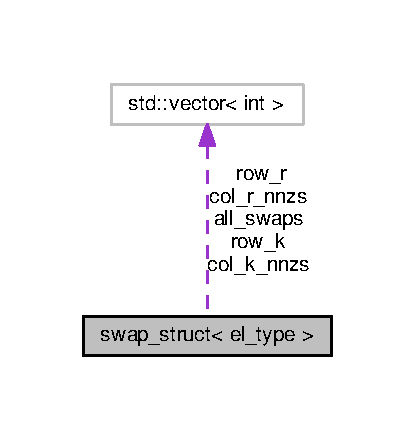
\includegraphics[width=199pt]{classswap__struct__coll__graph}
\end{center}
\end{figure}
\subsection*{Public Member Functions}
\begin{DoxyCompactItemize}
\item 
void \hyperlink{classswap__struct_ac67fad73735b183c372ef63b4a9cd581}{swap\+\_\+clear} ()\hypertarget{classswap__struct_ac67fad73735b183c372ef63b4a9cd581}{}\label{classswap__struct_ac67fad73735b183c372ef63b4a9cd581}

\begin{DoxyCompactList}\small\item\em Clears all swap vectors (swapk, swapr, all\+\_\+swaps). \end{DoxyCompactList}\item 
void \hyperlink{classswap__struct_ad97200ee23cd1f70668d6b4462228343}{col\+\_\+clear} ()\hypertarget{classswap__struct_ad97200ee23cd1f70668d6b4462228343}{}\label{classswap__struct_ad97200ee23cd1f70668d6b4462228343}

\begin{DoxyCompactList}\small\item\em Clears all col vectors (col\+\_\+k, col\+\_\+r, col\+\_\+k\+\_\+nnzs, col\+\_\+r\+\_\+nnzs). \end{DoxyCompactList}\item 
void \hyperlink{classswap__struct_a9727bf8ea70308977661235c59e3b8da}{row\+\_\+clear} ()\hypertarget{classswap__struct_a9727bf8ea70308977661235c59e3b8da}{}\label{classswap__struct_a9727bf8ea70308977661235c59e3b8da}

\begin{DoxyCompactList}\small\item\em Clears all row vectors (row\+\_\+k, row\+\_\+r). \end{DoxyCompactList}\end{DoxyCompactItemize}
\subsection*{Public Attributes}
\begin{DoxyCompactItemize}
\item 
vector$<$ idx\+\_\+it $>$ \hyperlink{classswap__struct_a609dd0d32e04b30b0db6830ab56a8de9}{swapk}\hypertarget{classswap__struct_a609dd0d32e04b30b0db6830ab56a8de9}{}\label{classswap__struct_a609dd0d32e04b30b0db6830ab56a8de9}

\begin{DoxyCompactList}\small\item\em List of indices from row r that will be swapped to row k. \end{DoxyCompactList}\item 
vector$<$ idx\+\_\+it $>$ \hyperlink{classswap__struct_a145f164cc7d5b81b259f0fe558faacf9}{swapr}\hypertarget{classswap__struct_a145f164cc7d5b81b259f0fe558faacf9}{}\label{classswap__struct_a145f164cc7d5b81b259f0fe558faacf9}

\begin{DoxyCompactList}\small\item\em List of indices from row k that will be swapped to row r. \end{DoxyCompactList}\item 
idx\+\_\+vector\+\_\+type \hyperlink{classswap__struct_af5461fcf0c0808ef0ef5ac9c6e212839}{all\+\_\+swaps}\hypertarget{classswap__struct_af5461fcf0c0808ef0ef5ac9c6e212839}{}\label{classswap__struct_af5461fcf0c0808ef0ef5ac9c6e212839}

\begin{DoxyCompactList}\small\item\em Column indices of all swaps done in swapk and swapr. \end{DoxyCompactList}\item 
idx\+\_\+vector\+\_\+type \hyperlink{classswap__struct_a7a9e67b4e6e1b9d1e6d2aefef3edda71}{col\+\_\+k\+\_\+nnzs}\hypertarget{classswap__struct_a7a9e67b4e6e1b9d1e6d2aefef3edda71}{}\label{classswap__struct_a7a9e67b4e6e1b9d1e6d2aefef3edda71}

\begin{DoxyCompactList}\small\item\em Row indices of non-\/zeros in the new column k. \end{DoxyCompactList}\item 
idx\+\_\+vector\+\_\+type \hyperlink{classswap__struct_a8d4e30cd03fc142b81a332db04edc244}{col\+\_\+r\+\_\+nnzs}\hypertarget{classswap__struct_a8d4e30cd03fc142b81a332db04edc244}{}\label{classswap__struct_a8d4e30cd03fc142b81a332db04edc244}

\begin{DoxyCompactList}\small\item\em Row indices of non-\/zeros in the new column r. \end{DoxyCompactList}\item 
elt\+\_\+vector\+\_\+type \hyperlink{classswap__struct_a39ab00a67015a67c375b620f54cc6352}{col\+\_\+k}\hypertarget{classswap__struct_a39ab00a67015a67c375b620f54cc6352}{}\label{classswap__struct_a39ab00a67015a67c375b620f54cc6352}

\begin{DoxyCompactList}\small\item\em Non-\/zero values in the new column k (order dependent on col\+\_\+k\+\_\+nnzs). \end{DoxyCompactList}\item 
elt\+\_\+vector\+\_\+type \hyperlink{classswap__struct_a3803a938141694098700de00d5cb6a7d}{col\+\_\+r}\hypertarget{classswap__struct_a3803a938141694098700de00d5cb6a7d}{}\label{classswap__struct_a3803a938141694098700de00d5cb6a7d}

\begin{DoxyCompactList}\small\item\em Non-\/zero values in the new column r (order dependent on col\+\_\+r\+\_\+nnzs). \end{DoxyCompactList}\item 
idx\+\_\+vector\+\_\+type \hyperlink{classswap__struct_a52180e1635646cd4f2dab0209ae62cb9}{row\+\_\+k}\hypertarget{classswap__struct_a52180e1635646cd4f2dab0209ae62cb9}{}\label{classswap__struct_a52180e1635646cd4f2dab0209ae62cb9}

\begin{DoxyCompactList}\small\item\em Column indices of non-\/zeros in the new row k. \end{DoxyCompactList}\item 
idx\+\_\+vector\+\_\+type \hyperlink{classswap__struct_a3b6ad04f7393ddd5c8b130e33208d427}{row\+\_\+r}\hypertarget{classswap__struct_a3b6ad04f7393ddd5c8b130e33208d427}{}\label{classswap__struct_a3b6ad04f7393ddd5c8b130e33208d427}

\begin{DoxyCompactList}\small\item\em Column indices of non-\/zeros in the new row r. \end{DoxyCompactList}\end{DoxyCompactItemize}


\subsection{Detailed Description}
\subsubsection*{template$<$class el\+\_\+type$>$\\*
class swap\+\_\+struct$<$ el\+\_\+type $>$}

A structure containing variables used in pivoting a L\+I\+L-\/C matrix. 

Storing these variables in a combined structure reduces memory requirements and bundles together all temporary structures needed during pivoting. 

The documentation for this class was generated from the following file\+:\begin{DoxyCompactItemize}
\item 
source/swap\+\_\+struct.\+h\end{DoxyCompactItemize}

%--- End generated contents ---

% Index
\backmatter
\newpage
\phantomsection
\clearemptydoublepage
\addcontentsline{toc}{chapter}{Index}
\printindex

\end{document}
